\chapter{\modif{Algorithme de segmentation interactive Superpixel $\alpha$-Fusion}}

\section{Introduction}
L'une des \modif{principales} contributions \modif{présentée dans ce mémoire est} la proposition d'une nouvelle méthode de segmentation interactive, $S \alpha F$ (Superpixel $\alpha$-Fusion) \cite{mathieu2016segmentation, mathieu2017jei}. Cette méthode permet la sélection précise, intuitive et rapide de multiples objets au sein d'une même photographie. Elle appartient à la catégorie des algorithmes de segmentation interactive \modif{multiclasse} et repose sur une approche par recherche des régions. Les germes donnés par l'utilisateur correspondent à des traits de couleur qui indiquent quelques pixels appartenant à chaque objet à extraire. 

L'algorithme $S \alpha F$ repose sur la modélisation du problème de la segmentation interactive comme la minimisation d'une fonction \modif{de coût} pouvant être représentée par un graphe de facteurs. Il intègre l'utilisation d'une méthode de classification par apprentissage supervisé assurant l'adéquation entre la segmentation produite et les germes donnés, l'introduction d'un nouveau terme de régularisation et la réalisation d'un pré-traitement consistant à regrouper les pixels en petits ensembles cohérents. 

\section{Modélisation du problème de segmentation interactive }

Soit $I$ une image, $\mathbb{S}=\lbrace \mathbf{s}_{1}, \cdots, \mathbf{s}_{N_{\mathbb{S}}} \rbrace$ un ensemble de $N_{\mathbb{S}}$ primitives visuelles, \modif{$\Lambda= \lbrace\lambda_{1},\cdots,\lambda_{N_\Lambda} \rbrace$} un ensemble de \modif{$N_{\Lambda}$} labels correspondant à \modif{$N_{\Lambda}$} classes et $G=\lbrace g_{1}, \cdots, g_{N_{G}} \rbrace$ un ensemble de germes indiquant pour chaque classe quelques pixels lui appartenant. Nous nous intéressons au problème consistant à attribuer, à chaque pixel de $I$, un élément de \modif{$\Lambda$} sous les contraintes suivantes :
\begin{itemize}
\item les pixels possédant le même label doivent former un ensemble visuellement homogène ;
\item la classification produite doit être cohérente vis-à-vis de $G$.
\end{itemize}

Dans le cadre de l'algorithme que nous proposons, chaque primitive visuelle $\mathbf{s}_{i}$ est un ensemble de pixels voisins et similaires,  nommé \emph{superpixel}. Ces ensembles sont construits de manière à ce que l'attribution d'une et \modif{d'}une seule classe à chaque superpixel permette d'obtenir la segmentation recherchée par l'utilisateur.

Les superpixels forment une partition en composantes connexes des pixels de l'image $I$. Ils peuvent donc être représentés par un \modif{graphe} $\mathcal{G}=\ <X,E>$, avec :
\begin{itemize}
\item $X = \lbrace x_{1}, \cdots, x_{N_{\mathbb{S}}}  \rbrace$  un ensemble de sommets, où chaque sommet $x_{i}$ représente un superpixel $ \mathbf{s}_{i}$ ;
\item $E$ un ensemble d'arêtes non orientées, avec une arête $e_{i,j}$ pour chaque paire de superpixels $(\mathbf{s}_{i},\mathbf{s}_{j})$ ayant des pixels \modif{voisins}. 
\end{itemize}

Soit $C=\lbrace c_{1},\cdots,c_{\mathbb{S}} \rbrace$, un ensemble de variables aléatoires indexées par les sommets de $\mathcal{G}$, tel que \modif{$c_{i} \in \Lambda$}. Si nous admettons que la probabilité d'une variable $c_{i}$ de recevoir le label $\lambda_{k}$ ne dépend que des caractéristiques des sommets $x_{j}$ voisins directs de $x_{i}$, alors \modif{$C$} est un \modif{champ aléatoire de Markov} (CAM) et une segmentation optimale \modif{$C^{*}$} s'obtient en minimisant : \modif{
\begin{equation}
\label{eq:safe:mrfprob}
\mathcal{F}_{CAM} (I,C,G) = \sum_{i=1}^{N} \mathcal{F}_{D}(x_{i},c_{i}) \ + \sum_{ e_{i,j} \in E} \omega(x_{i})\mathcal{F}_{R}(x_{i},c_{i},x_{j},c_{j})
\end{equation}}
avec :
\begin{itemize}
\item $\mathcal{F}_{D}$ un terme d'attache aux données, s'assurant de la cohérence \modif{avec les} caractéristiques  \modif{de l'image} $I$ et \modif{celles} des germes $G$ ;
\item $\mathcal{F}_{R}$ un terme de régularisation vérifiant certaines propriétés propres à la segmentation, concernant par exemple  la taille \modif{ou la forme} des régions ;
\item  $\omega$  une fonction de pondération.
\end{itemize}

\subsection{Terme d'attache aux données}

Une segmentation optimale \modif{$C^{*}$} de $I$ étant obtenue par minimisation de $\mathcal{F}_{CAM}$, le terme d'attache aux données \modif{$\mathcal{F}_{D}$} \modif{vaut :} 
\modif{
\begin{equation}
 \mathcal{F}_{D}(x_{i},c_{i}) = 1 -P(\lambda_{j}|x_{i} ) \text{ avec } c_{i} =  \lambda_{j}\text{.} 
\end{equation}
où $P(\lambda_{j}|x_{i} )$ est la probabilité que le sommet $x_{i}$ appartiennent à la classe de label $\lambda_{j}$.
}

\subsubsection{Approche de Wu}
Comme nous nous intéressons à un problème de classification \modif{multiclasse}, \modif{$P(\lambda_{j}|x_{i})$} peut être estimée de manière précise grâce à la seconde des deux méthodes décrites par Wu \textit{et al.}, dans leur article \emph{\og Probability estimates for multi-class classification by pairwise coupling \fg} \cite{wu2004probability}. Elle s'appuie sur le résultat d'une méthode de classification supervisée résolvant des problèmes à deux classes. La fonction binaire associée à cette méthode est $F_{sup}(x_{i},\lambda_{j},\lambda_{k})$ qui vaut :
\begin{itemize}
\item $0$ si les caractéristiques de $x_{i}$ sont plus \modif{proches} \modif{de celles} de la classe $\lambda_{j}$ ;
\item $1$ si les caractéristiques de $x_{i}$ sont plus \modif{proches}  \modif{de celles} de la classe $\lambda_{k}$.
\end{itemize}
L'estimation de la  probabilité que $x_{i}$ appartienne à la classe de label $\lambda_{j}$ plutôt qu'à la classe de label $\lambda_{k}$ est obtenue en calculant :
\modif{
\begin{equation}
F_{jk}(x_{i},\lambda_{j},\lambda_{k}) = \dfrac{1}{1+ \exp(\omega_{A} F_{sup}(x_{i},\lambda_{j},\lambda_{k}) +\omega_{B})}
\end{equation}}
où $\omega_{A}$ et $\omega_{B}$ sont deux paramètres obtenus lors de la phase d'apprentissage de la méthode de classification supervisée. À partir de cette probabilité, Wu \textit{et al.} montrent que la distribution de probabilité \modif{$\mathcal{P}= \lbrace P(\lambda_{1}|x_{i} ), \cdots ,P(\lambda_{N_{\Lambda}}|x_{i} )  \rbrace$} s'estime en minimisant :
\modif{
\begin{equation}
\sum_{j=1}^{N_{\Lambda}} \sum_{\substack{k=1 \\ j \neq k}}^{N_{\Lambda}} \Big( F_{jk}(x_{i},\lambda_{j},\lambda_{k}) P(\lambda_{k}|x_{i} ) - F_{kj}(x_{i},\lambda_{j},\lambda_{k}) P(\lambda_{j}|x_{i} ) \Big)^{2}
\end{equation}
sous les contraintes suivantes :
\begin{itemize}
\item $\displaystyle \sum_{j=1}^{N^{\Lambda}} P(\lambda_{j}|x_{i} ) = 1 $;
\item $P(\lambda_{j}|x_{i} ) \text{ } >0 \ \forall\ j \ \in [1,N_{\Lambda}]$.
\end{itemize}}

\subsubsection{Classification supervisée}
L'utilisation d'une méthode de classification supervisée implique de disposer d'un ensemble de \emph{données d'apprentissage}, permettant de paramétrer la méthode, afin que celle-ci puisse classer les données restantes, nommées \emph{données d'exploitation}. Dans le cas de la méthode que nous proposons, il s'agit de produire une partition de l'ensemble des superpixels \modif{$\mathbb{S}$} associé à une image en deux ensembles : 
\begin{itemize}
\item \modif{$\mathbb{S}_{A}$} pour les données d'apprentissage ;
\item \modif{$\mathbb{S}_{E}$} pour les données d'exploitation.
\end{itemize}
La construction de ces deux ensembles s'effectue par analyse des indications données par l'utilisateur. L'ensemble des germes $G$ étant constitué de couples $(p_{i},\lambda_{j})$, associant un label à certains pixels de l'image $I$, il convient de trouver une procédure à la fois rapide et fiable pour transférer ces germes vers les superpixels. 

Soit $\mathbf{s}_{k}$ un superpixel. Trois cas de figure peuvent se présenter :
\begin{enumerate}
\item $\mathbf{s}_{k}$ ne contient aucun pixel correspondant à un germe \modif{c'est-à-dire} $\nexists (p_{i},\lambda_{j}) \in G \text{, } p_{i} \in \mathbf{s}_{k}$ ;
\item $\mathbf{s}_{k}$ contient des germes \modif{de} plusieurs classes, \modif{c'est-à-dire} ${\exists (p_{i1},\lambda_{j1}) \in G \land   (p_{i2},\lambda_{j2}) \in G \text{, } }\\{p_{i1} \in \mathbf{s}_{k} \land  p_{i2} \in \mathbf{s}_{k} \land  \lambda_{j1} \neq \lambda_{j2}}$ ;
\item $\mathbf{s}_{k}$ contient des germes d'une seule classe, de label \modif{$\lambda_{l}$, c'est-à-dire que $ (p_{i},\lambda_{j}) \in G  \land  p_{i} \in \mathbf{s}_{k} \implies \lambda_{j} =  \lambda_{l}$}.
\end{enumerate}
Nous avons choisi d'utiliser uniquement les superpixels de la troisième catégorie pour constituer l'ensemble \modif{$\mathbb{S}_{A}$}  et de considérer les superpixels du deuxième type comme étant des données erronées. 

Les méthodes de classification supervisée de type \modif{séparateur à vaste marge (SVM)} et de type FA sont traditionnellement utilisées avec l'approche décrite par Wu \textit{et al.} \cite{wu2004probability}. La section \ref{sec:saf:SelectClassifSup} \modif{présente notre démarche} pour sélectionner la plus pertinente dans le cadre d'une d'application de segmentation interactive. 
 
\subsection{Terme de régularisation}

La segmentation obtenue par la seule minimisation du terme d'attache aux données $\mathcal{F}_{D}$ peut, dans certains cas, contenir de nombreuses erreurs qui se présentent sous la forme de superpixels \modif{attribués à la mauvaise classe}, alors que l'ensemble de leurs voisins a été classé correctement. Nous parlons alors de segmentation \emph{bruitée}, par analogie avec le bruit présent dans les images, au niveau des pixels. 

Ce bruit complique considérablement la tâche de l'utilisateur, qui doit rajouter de nombreux germes pour le corriger. La méthode la plus courante pour s'en prémunir consiste à intégrer, comme nous l'avons fait, un terme de régularisation au sein de la fonction \modif{de coût} à minimiser. Les termes de régularisation généralement \modif{utilisés} favorisent la production d'une segmentation dont les régions sont \modif{grandes}, de formes régulières, avec des contours suivant les bordures des objets présents dans l'image. \modif{La prise en compte de ce} type d'\textit{a priori} sur les régions composant une segmentation optimale présente cependant le désavantage d'augmenter significativement le temps d'exécution de la méthode \cite{mille2015combination, santner2010interactive}. 

Nous proposons un nouveau terme de régularisation dont les objectifs sont les suivants :
\begin{itemize}
\item réduire le bruit au sein de la segmentation ;
\item conserver une complexité algorithmique suffisamment faible pour garantir une méthode fonctionnant en temps interactif ;
\item préserver les classes rares.
\end{itemize}

Par \emph{temps interactif} nous entendons un temps d'exécution de quelques secondes maximum pour des images de plusieurs millions de pixels, prérequis nécessaire pour que la méthode soit adoptée par un utilisateur.

Une classe est dite \emph{ rare} si elle correspond à un petit objet, peu représenté en termes de nombre de superpixels. Les classes rares se révèlent problématiques car elles présentent de nombreux aspects communs avec le bruit présent dans la segmentation. Ces classes rares prennent la forme de quelques superpixels entourés de superpixels attribués à une autre classe. La figure \ref{fig:saf:classesRares} illustre notre propos. Sur l'image d'origine (voir \modif{la} figure \ref{fig:saf:classesRares}a), les objets visibles se répartissent en trois classes : deux classes majoritaires (en noir et rose) et une classe rare (en bleu). La figure \ref{fig:saf:classesRares}b montre une segmentation obtenue. Cette segmentation est bruitée, l'un des superpixels de la classe noire ayant été attribué par erreur à la classe rose. 

L'analyse de cet exemple nous donne une piste pour la résolution du problème qui nous occupe. En effet, même si la segmentation obtenue sur la figure \ref{fig:saf:classesRares}b est bruitée, nous pouvons constater qu'il est plus fréquent pour un superpixel attribué à la classe bleue d'avoir comme voisin un superpixel de la classe noire, que pour un superpixel de la classe rose. Ainsi la probabilité $P_{i}(j)$ pour un superpixel de classe de label $\lambda_{i}$ d'avoir comme voisin un superpixel attribué à la classe de label $\lambda_{j}$, fournit une information permettant de distinguer un superpixel appartenant à une classe rare d'un superpixel bruité.

\begin{figure}[htb]
	\centering
	 \begin{subfigure}[t]{0.45\textwidth}	
			
\includegraphics[width=\textwidth]{images/saf/ex_f_reg_im}
		 \caption{\modif{Image originale}. Trois classes sont présentes : deux classes majoritaires (en noir et rose) et une classe rare (en bleu). }
	\end{subfigure}		
	~
	 \begin{subfigure}[t]{0.45\textwidth}	
			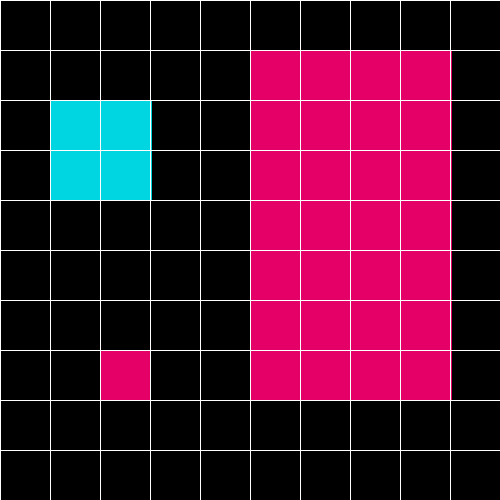
\includegraphics[width=\textwidth]{images/saf/ex_f_reg_seg}
		 \caption{Segmentation erronée : l'un des superpixels de \modif{la} classe noire a été attribué par erreur à la classe rose. Les contours des superpixels sont tracés en blanc.}
	\end{subfigure}	
	\caption{Distinction entre classes rares et erreurs de segmentation.}
	\label{fig:saf:classesRares}
\end{figure}

Soit $\mathbf{s}_{i}$ un superpixel, $x_{i}$ le sommet qui lui est associé et \modif{$\mathcal{P}= \lbrace P(\lambda_{1}|x_{i} ), \cdots, P(\lambda_{N_{\Lambda}}|x_{i} )  \rbrace$} l'ensemble des probabilités que ce superpixel appartienne à chacune des classes. La classe de \modif{label} $\lambda_{j}$ est attribuée à $x_{i}$ de manière à ce que :
\begin{equation}
P(\lambda_{j}|x_{i} )  \geqslant  P(\lambda_{k} | x_{i})\  \forall  k \in [1,N_{\Lambda}] \text{.}
\end{equation}
Après avoir ainsi obtenu une première segmentation, la probabilité $P_{i}(j)$ s'obtient rapidement en calculant l'histogramme normalisé des classes des superpixels voisins d'un superpixel de label $\lambda_{i}$. Soulignons que, du fait qu'une distribution de probabilité soit calculée pour chacune des classes $P_{i}(j) \neq P_{j}(i)$. Comme les arêtes de $\mathcal{G}$ sont non orientées, $P_{i}(j)$ et $P_{j}(i)$ \modif{doivent être fusionnées}. Nos tests ont montré que :
\begin{equation}
\mathcal{F}_{R}(x_{i},c_{i},x_{j},c_{j})= 1-\max(P_{i}(j),P_{j}(i))
\end{equation}
donne de bons résultats. \modif{L'utilisation de la fonction moyenne ou de la fonction minimum, à la place de la fonction maximum, ne permet pas d'améliorer la qualité des segmentations produites par $S \alpha F$}.

\subsection{Fonction de pondération}
La fonction de pondération $\omega$ dose l'influence du terme de régularisation par rapport au terme d'attache aux données. Dans la fonction \modif{de coût} définie par l'équation \ref{eq:safe:mrfprob}, le terme d'attache aux données intervient une fois par sommet, tandis que le terme de régularisation contribue à augmenter \modif{la valeur de la fonction} pour chaque arête, c'est-à-dire pour chaque couple de \modif{sommets} voisins. \modif{Pour que la contribution de la somme des termes de régularisation rattachés à un même sommet soit similaire quel que soit le nombre de voisin d'un sommet, il est} nécessaire que la fonction de pondération intègre \modif{le nombre de voisins de ce sommet. Soit $\nei(x_{i})$, la fonction renvoyant l'ensemble des sommets voisins de $x_{i}$.} Plusieurs tests nous ont conduit à sélectionner la fonction suivante :
\modif{
\begin{equation}
\omega (x_{i}) = \frac{\nombre{0,7}}{|\nei(x_{i})|}\text{.}
\end{equation}
}

\subsection{Algorithme $S \alpha F$ }

L'objectif de l'algorithme $S \alpha F$ consiste à minimiser la fonction $\mathcal{F}_{CAM}$. La figure \ref{fig:saf:algo} en schématise le fonctionnement général. 

L'approche $S \alpha F$ comprend une étape d'\emph{initialisation}, qui permet d'extraire les \modif{superpixels}, et une étape de \emph{segmentation}, où les germes donnés par l'utilisateur sont pris en compte. Tandis que l'étape d'initialisation ne nécessite d'être réalisée qu'une seule fois, l'étape de segmentation est répétée tant que l'utilisateur modifie les germes. 

Lors de l'étape d'initialisation, les pixels sont d'abord groupés en superpixels. Les \modif{caractéristiques} de chaque superpixel sont ensuite analysées et un descripteur sous la forme d'un vecteur à $N_{d}$ dimensions est calculé. Ainsi\modif{,} le nombre de primitives visuelles se voit considérablement réduit, chaque superpixel regroupant plusieurs centaines de pixels, ce qui accèlere les traitements effectués lors de l'étape de segmentation. 

Cette dernière concerne la minimisation à proprement parler de $\mathcal{F}_{CAM}$ et se déroule de la manière suivante :

\begin{enumerate}
\item les germes donnés par l'utilisateur sont analysés afin d'obtenir :
\begin{enumerate}
\item le nombre de classes $N_{\Lambda}$ ;
\item pour chaque classe, l'ensemble \modif{$\mathcal{S}_{A}^{\lambda_{i}}$ des superpixels nécessaires} pour entraîner la méthode de classification à reconnaître les superpixels appartenant à cette classe ;
\end{enumerate}
\item à l'aide de la méthode de classification, la probabilité de chaque superpixel d'appartenir à chacune des classes est calculée ;
\item l'obtention de ces probabilités permet de calculer\modif{,} pour chaque superpixel, le terme d'attache aux données \modif{$\mathcal{F}_{D}$} ;
\item une première segmentation est produite en attribuant à chaque superpixel la classe la plus probable ;
\item cette segmentation est analysée afin d'obtenir pour chaque couple de classes $(\lambda_{i}, \lambda_{j})$ les probabilités \modif{$P_{i}(j)$ et $P_{j}(i)$} ;
\item l'obtention de ces probabilités permet de calculer pour chaque paire de superpixels voisins le terme de régularisation \modif{$\mathcal{F}_{R}$} ;
\item une approximation de la segmentation correspondant à la valeur minimale de \modif{$\mathcal{F}_{CAM}$} est recherchée ;
\item le label attribué à chaque superpixel est transféré à l'ensemble des pixels le constituant ;
\item la segmentation résultat est montrée à l'utilisateur qui peut éventuellement ajouter ou supprimer des germes. 
\end{enumerate}

\begin{figure}[htbp]
\begin{center}
\scalebox{.5}{
\input{images/saf/algoOverview.pdf_t}
}
\caption{Schéma général de l'algorithme $S \alpha F$.}
\label{fig:saf:algo}
\end{center}
\end{figure}

À partir de cet algorithme général, toute une famille de méthodes peuvent être obtenues, dont les variations tiennent dans le choix de la méthode de sur-segmentation, des \modif{caractéristiques utilisées} pour décrire chaque superpixel, de la méthode de classification par apprentissage supervisé et de l'algorithme d'optimisation permettant de minimiser la fonction \modif{de coût}.

\section{Algorithme de sur-segmentation}

\subsection{Problématique}
L'algorithme de sur-segmentation utilisé doit permettre de regrouper rapidement les pixels de l'image en superpixels, de manière à minimiser la probabilité qu'un superpixel chevauche deux objets différents. L'obtention des superpixels ainsi que le \modif{calcul} de leurs descripteurs n'est réalisé qu'une seule fois, lors de l'étape d'initialisation. Comme la même classe est attribuée à l'ensemble de ses pixels, un superpixel contenant des pixels appartenant à deux éléments que l'utilisateur souhaite séparer engendrera des erreurs dans la segmentation résultat. \modif{Quel que} soit le nombre de germes ajoutés par l'utilisateur, cette erreur ne pourra pas être corrigée, puisqu'aucun mécanisme ne permet de séparer le superpixel en deux nouveaux superpixels. 

Le choix d'un algorithme de sur-segmentation est donc une étape clé pour le bon fonctionnement de $S \alpha F$. Suite à une \modif{évaluation des principales méthodes} existantes (qui fait l'objet du \modif{chapitre 4}), nous avons choisi l'algorithme SLIC (\og \textit{Simple Linear Iterative Clustering} \fg) \cite{achanta2012slic} qui fournit un bon compromis entre qualité du résultat et rapidité.

\subsection{Principe général de l'algorithme \modif{SLIC} et choix des paramètres} 

Proposé par Achanta \textit{et al.}  SLIC \cite{achanta2012slic}, est \modif{une} version modifiée de l'algorithme de $k$-moyennes. Des superpixels initiaux sont produits en regroupant les pixels selon une grille régulière. Le choix de taille des cases est un paramètre qu'il convient de fixer, soit en précisant un nombre souhaité de superpixels (les pixels de l'image sont alors découpés en autant de case que nécessaire), soit en précisant l'aire moyenne désirée pour les superpixels (la hauteur et la largeur des cases sont alors \modif{déterminées} pour s'approcher le plus possible de cette aire). 

L'algorithme SLIC répète alors une dizaine de fois les  deux étapes suivantes :
\begin{enumerate}
\item la couleur et la localisation \modif{moyennes} de chaque superpixel sont calculées ;
\item chaque pixel est rattaché au superpixel maximisant une fonction de similarité.
\end{enumerate}

L'une des contributions essentielles d'Achanta \textit{et al.} concerne la fonction permettant de mesurer la similarité entre un pixel et un superpixel. Cette dernière fait intervenir à la fois la couleur et la localisation. Un paramètre, fixé par l'utilisateur, permet de pondérer l'influence de chacune de ces deux informations.  

Une dernière étape permet d'uniformiser la taille des superpixels et de s'assurer que ces derniers correspondent bien à des composantes connexes.

Les deux paramètres \modif{à fixer} pour cette méthode sont donc \modif{:}
\begin{itemize}
\item le nombre de \modif{superpixels}, que nous avons fixé à $3000$\modif{, afin d'obtenir des superpixels suffisamment petits pour réduire les erreurs dans la sur-segmentation} ;
\item le poids pour la fonction de similarité, pour lequel Achanta \textit{et al.} \cite{achanta2012slic} recommandent une valeur de $10$\modif{,} ce qui s'est avéré pertinent dans le cas de $S \alpha F$.
\end{itemize}

Une description détaillée de l'algorithme SLIC est donnée \modif{dans la section} \ref{subsec:sp:slic}. La section \ref{subsec:sp:res-slic} contient, \modif{quant à} elle, une analyse des qualités nous ayant conduit à le choisir. 

\section{Description des superpixels }

\subsection{Problématique}

Les superpixels correspondant à des ensembles homogènes de pixels connexes, les descripteurs qui caractérisent leur apparence peuvent au choix, soit tirer partie de la diversité de l'information contenue dans un superpixel, soit chercher à la résumer. Les descripteurs de la première catégorie comprennent par exemple :
\begin{itemize}
\item les histogrammes \modif{des} différents canaux de \modif{couleur} ;
\item \modif{l'histogramme} d'un descripteur de texture tel que les textons ou les motifs binaires locaux \cite{pietikainen2011local} (LBP, de l'anglais \modif{\og \emph{Local Binary Patterns} \fg}).
\end{itemize}

Pour la seconde catégorie, nous trouvons\modif{,} entre autres :
\begin{itemize}
\item la moyenne \modif{de} chaque canal de couleur  ; 
\item l'écart type \modif{de} chaque canal de couleur  ;
\item le coefficient de dissymétrie  \modif{de} chaque canal de couleur ; 
\item le kurtosis \modif{de} chaque canal de couleur  ; 
\item la position du barycentre ;
\item l'aire en nombre de pixels ;
\item le rapport entre l'aire \modif{du superpixel} et celle du plus petit rectangle l'englobant. 
\end{itemize}

Les descripteurs choisis doivent permettre de regrouper les superpixels appartenant à la même classe, tout en séparant ceux \modif{correspondant} à des objets différents. \modif{Ne disposant d'aucune connaissance \textit{a priori} sur l'image}, ni sur les propriétés de la segmentation que l'utilisateur voudra obtenir, ils doivent également s'adapter à un large panel de situations. Enfin, ni leur extraction durant l'étape \modif{d'initialisation, }ni leur utilisation durant l'étape de segmentation ne doivent se répercuter de manière trop importante sur les temps d'exécution. 

Certaines caractéristiques, notamment celles associées à la texture, requièrent un nombre de calculs élevé lors de l'étape d'initialisation. Par ailleurs, plus le descripteur contient de caractéristiques, plus le temps nécessaire \modif{pour évaluer} la probabilité d'un superpixel d'appartenir à chacune des classes est important. 

\subsection{Choix d'un descripteur}

Nous avons choisi un descripteur \modif{minimaliste} comprenant cinq caractéristiques :
\begin{itemize}
\item trois pour exprimer la couleur moyenne du superpixel dans l'espace colorimétrique RGB ;
\item deux pour exprimer sa localisation dans l'image, \modif{par} les coordonnées de son barycentre.
\end{itemize} 

Ces cinq caractéristiques sont normalisées : pour la couleur, nous divisons chaque moyenne par $255$ \modif{;} pour les coordonnées du barycentre\modif{,} nous divisions l'abscisse par la largeur de l'image et l'ordonnée par la hauteur de l'image. Nous obtenons un descripteur rapide à calculer lors de la phase d'initialisation et comprenant peu de caractéristiques, ce qui accélère son utilisation lors de l'étape de segmentation.  

L'information de couleur permet de segmenter rapidement et avec un minimum de germes de larges zones homogènes telles que le ciel. Lorsque l'utilisateur souhaite séparer deux objets ayant des teintes similaires, l'information de localisation prend le relais. Cette dernière assure également que les germes conservent un comportement local c'est-à-dire que l'ajout de germes sur une partie de l'image ne perturbe pas la segmentation dans le reste de la photographie.


\begin{emodif}
\subsection{Problèmes liés au positionnement des germes}
\label{subsec:eval:posgermes}

En contrepartie des deux qualités de ce descripteur -- sa rapidité et l'influence intuitive des germes -- la simplicité de ce dernier fait que, dans certains cas, les indications données par l'utilisateur peuvent ne pas être suffisantes pour trouver une segmentation pertinente de l'image. 

Tout d'abord, les germes peuvent ne pas être suffisants pour créer un modèle des objets à extraire pertinent en termes de couleur. Un exemple est présenté sur la figure \ref{fig:eval:Algo-fails-c}. Le pollen de cette dernière, en jaune, n'est pas correctement segmenté. Aucun pixel jaune n'étant sélectionné comme germe, cette teinte est rattachée à tort au fond, dont la couleur verte est plus proche du jaune que du rouge des pétales de la fleur. L'ajout de quelques germes sur l'une des deux zones centrales des fleurs suffit à améliorer netteent la qualité de la segmentation. 
 
\begin{figure}[htb]
 \centering
 \begin{subfigure}{0.4\textwidth}	
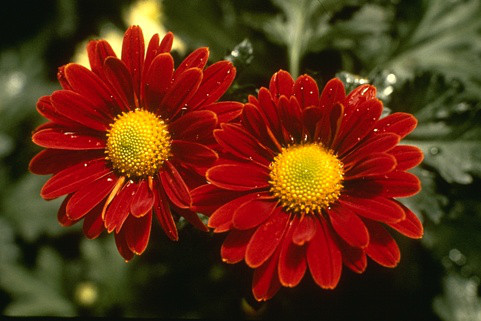
\includegraphics[width=\textwidth]{images/evaluation/fails/im_c}
 \end{subfigure}
 \\~\\
 \begin{subfigure}{0.4\textwidth}	
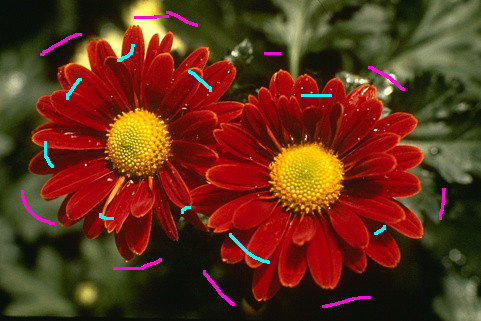
\includegraphics[width=\textwidth]{images/evaluation/fails/germes_c_01}
 \end{subfigure}
 ~
 \begin{subfigure}{0.4\textwidth}	

\includegraphics[width=\textwidth]{images/evaluation/fails/seg_c_01}
 \end{subfigure}
 \\~\\
 \begin{subfigure}{0.4\textwidth}	
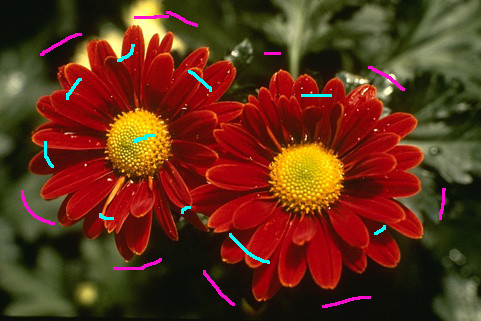
\includegraphics[width=\textwidth]{images/evaluation/fails/germes_c_02}
 \end{subfigure}
 ~
 \begin{subfigure}{0.4\textwidth}	

\includegraphics[width=\textwidth]{images/evaluation/fails/seg_c_02}
 \end{subfigure}
\caption{Illustration de l'impact de la répartition des germes en termes de couleur  sur la qualité de la segmentation obtenue.}
	\label{fig:eval:Algo-fails-c}
\end{figure} 

Inversement, les germes peuvent ne pas être répartis correctement dans l'image en termes de localisation, à l'instar de l'exemple donné sur la figure \ref{fig:eval:Algo-fails}. Ici, même si théoriquement la couleur devrait permettre de séparer correctement l'éléphant, le ciel et la végétation, l'utilisation d'une information de localisation vient perturber la méthode de classification pour la partie gauche de l'image qui, contrairement à la moitié droite, ne contient pas de germes. 

\begin{figure}[htb]
 \centering
 \begin{subfigure}{0.4\textwidth}	
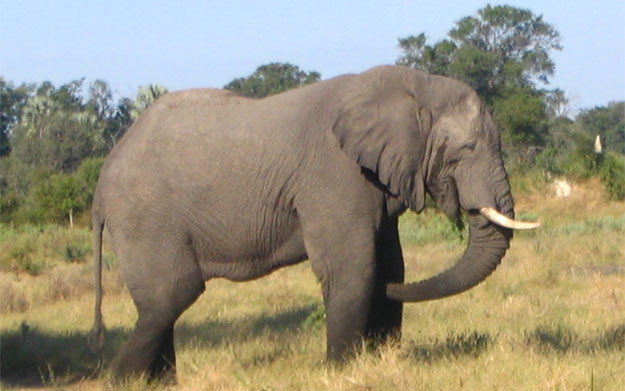
\includegraphics[width=\textwidth]{images/evaluation/fails/im}
 \end{subfigure}
 \\~\\
 \begin{subfigure}{0.4\textwidth}	
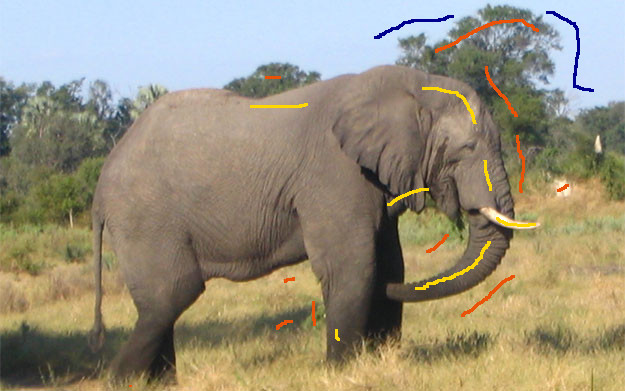
\includegraphics[width=\textwidth]{images/evaluation/fails/germes_01}
 \end{subfigure}
 ~
 \begin{subfigure}{0.4\textwidth}	

\includegraphics[width=\textwidth]{images/evaluation/fails/seg_01}
 \end{subfigure}
 \\~\\
 \begin{subfigure}{0.4\textwidth}	
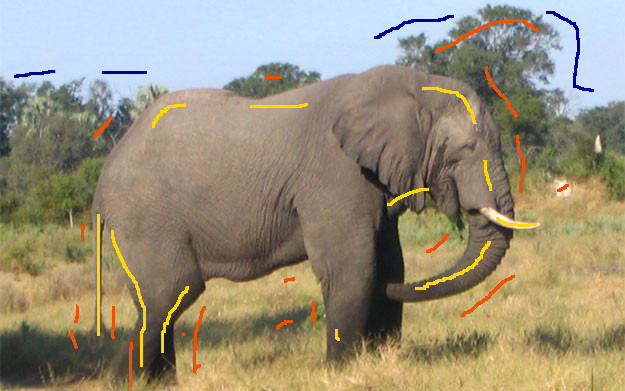
\includegraphics[width=\textwidth]{images/evaluation/fails/germes_02}
 \end{subfigure}
 ~
 \begin{subfigure}{0.4\textwidth}	
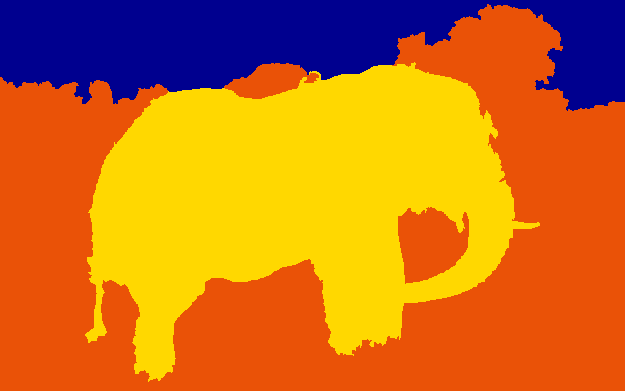
\includegraphics[width=\textwidth]{images/evaluation/fails/seg_02}
 \end{subfigure}
\caption{Illustration de l'impact de la répartition des germes \modif{en termes de localisation} sur la qualité de la segmentation obtenue.}
	\label{fig:eval:Algo-fails}
\end{figure} 

Afin d'éviter ce dernier problème, une consigne simple peut être donnée à l'utilisateur lui demandant de donner des germes \og \textit{près des contours}\fg. 

\end{emodif}

\subsection{Autres descripteurs testés }

En remplaçant  l'espace RGB par d'autres espaces colorimétriques (CIELab, HSV) nous n'avons pas constaté d'améliorations significatives. 

Il en va de même avec l'utilisation d'un descripteur de texture, dont le coût en termes de temps de calcul n'est pas compensé par une amélioration notable des performances (réduction du nombre de germes nécessaires et/ou diminution des erreurs dans la segmentation). Ainsi, nos tests avec les LBP, descripteur de texture pourtant à l'origine d'avancées notables dans de nombreux travaux en vision par ordinateur, ne nous ont pas permis d'améliorer les scores de précision de notre méthode.

L'utilisation des histogrammes de LBP s'est en revanche traduite par une augmentation du temps d'exécution de $23\%$ pour l'étape d'initialisation et de $76\%$ pour l'étape de segmentation. Ce résultat n'est  pas surprenant : les superpixels sont conçus sur la base de la couleur des pixels, de manière à former des ensembles homogènes. Ainsi, l'écart type moyen pour l'ensemble des données que nous avons utilisées ne dépasse pas les $4\%$, ce qui indique que les pixels au sein d'un même superpixel présentent peu de variations en termes de couleur.


\section{Choix d'une méthode de classification supervisée}
\label{sec:saf:SelectClassifSup}

L'approche de Wu \textit{et al.} \cite{wu2004probability}  est connue pour donner de bons résultats à la fois avec les méthodes de classification  SVM et  FA. Le choix de l'une de ces méthodes pour estimer la  probabilité qu'un superpixel appartienne à une classe, nécessite de s'intéresser aux forces et aux faiblesses de chacune d'entre elles, dans le cadre spécifique du problème de la segmentation interactive tel que nous l'avons posé. 

Ainsi, par rapport aux problèmes de classification par apprentissage canoniques, nous pouvons noter les particularités suivantes :
\begin{itemize}
\item nous disposons de peu de données d’apprentissage ;
\item de nombreuses images présentent des classes \emph{rares} ;
\item le descripteur  de chaque superpixel comprend peu de caractéristiques. 
\end{itemize}

Les données d'apprentissage étant spécifiques à une image, elles correspondent à un sous-ensemble des superpixels produits. Or, pour conserver des temps d'exécution raisonnables, le nombre de ces derniers ne doit pas dépasser \modif{ quelques milliers}. Si nous estimons que l'utilisateur annote environ $25 \%$ des superpixels, ce qui correspond déjà à un nombre élevé de germes et à un effort conséquent pour guider la méthode, nous disposons \modif{de} seulement quelques centaines de données d'apprentissage, à répartir entre les différentes classes. 

Parmi ces classes, certaines correspondent à de petits objets dont la surface en nombre de pixels est très inférieure à celles des autres composantes de l'image. \modif{Il est donc }probable que les données d'apprentissage pour ces classes soit moins nombreuses (quelques dizaines de superpixels).

Le fait que les descripteurs utilisés ne contiennent que cinq caractéristiques constitue également une singularité, de nombreux problèmes de classification ayant plutôt à faire face à un descripteur de taille trop importante, qu'il convient de réduire\modif{,} par exemple avec une analyse en composantes principales.

À ces spécificités inhérentes au contexte applicatif de la segmentation interactive, s'ajoutent celles liées à l'utilisation de la	 méthode de classification au sein de $S \alpha F$ et qui consiste à :
\begin{itemize}
\item estimer pour chaque superpixel une distribution de probabilité permettant de calculer le terme d'attache aux données ;
\item produire une segmentation initiale dont dépend la pertinence du terme de régularisation.
\end{itemize}

Le dernier point est sans doute le plus simple à évaluer : sachant la classe réelle d'un superpixel, il suffit de vérifier qu'elle correspond à sa classe prédite. Vérifier la qualité de la distribution de probabilité est plus \modif{délicat}. À partir de données de référence où chaque pixel est attribué à une classe, nous avons cherché à produire un nouvel ensemble de données de référence associant à chaque superpixel une distribution de probabilité de référence. Cela nous permet notamment de prendre en compte le fait qu'un superpixel en bordure d'un objet puisse avoir des caractéristiques proches de celles de plusieurs classes : dans ce cas de figure, nous préférons obtenir une distribution de probabilité témoignant de cette incertitude qu'une prédiction assurée pour l'une ou l'autre des classes. 

Enfin, soulignons que nos tests ont été réalisés à l'échelle du superpixel et non du pixel. En effet, un pixel se voit attribuer la classe du superpixel auquel il appartient. Les sources d'erreurs dans la segmentation présentes à cette échelle peuvent donc provenir soit d'une distribution de probabilité erronnée, soit d'une erreur commise par la méthode de sur-segmentation employée. Ici, seul le premier cas de figure nous intéresse. 

\subsection{Fonctionnement des deux méthodes}
\subsubsection{Séparateur à vaste marge}

Le principe \modif{d'un} SVM est illustré par la figure \ref{fig:saf:svm}. Il consiste à représenter une donnée comme un point dans un espace à $N_{D}$ dimensions et à lui attribuer une classe en fonction de sa position par rapport à un hyperplan. Pour déterminer la position de l’hyperplan, le classificateur SVM réalise une étape d’apprentissage durant laquelle il dispose de données déjà classées et cherche l’équation d’un hyperplan séparant les deux ensembles de points, de manière à maximiser l’écart $b$ entre les points périphériques (les vecteurs de support) et cet hyperplan de séparation. Si nous considérons nos données comme des vecteurs de $N_{d}$ éléments, un cas idéal serait celui où $N_{d} = N_{D}$. Concrètement, pour trouver un hyperplan séparant toutes les données, $N_{D}$ s’avère généralement très supérieur à $N_{d}$.

Il n’est pas toujours souhaitable que l’hyperplan sépare parfaitement l’ensemble des points : des points mal classés durant la phase d’apprentissage peuvent être tolérés afin de garantir qu’une marge entre les \modif{vecteurs de support} soit plus importante. Par exemple, dans le cas de la segmentation interactive, il est possible que l’utilisateur ait légèrement débordé lors de son tracé du germe, et qu’ainsi un superpixel soit attribué à tort à une classe. Il est intéressant que ces données d’apprentissage erronées puissent ne pas être prise en considération. Un paramètre  $\omega_{C}$ permet de pondérer l’importance des erreurs de classification par rapport
à celle de la largeur de la marge.


\begin{figure}[htb]
\begin{center}
\scalebox{.5}{
\input{images/saf/svm.pdf_t}
}
\caption{L’hyperplan optimal (en rouge), caractérisé par le vecteur $w$, avec la marge maximale $b$.
Les échantillons entourés en vert sont des \modif{vecteurs de support}. Les échantillons entourés en rouge sont des
erreurs tolérées lors de la phase d’apprentissage.}
\label{fig:saf:svm}
\end{center}
\end{figure}

L’évaluation de la distance entre deux points, dans un espace à $N_{D}$ dimensions, est réalisé au moyen d’une fonction nommée noyau. Pour le problème de segmentation interactive que nous cherchons à résoudre, nous avons utilisé le noyau \modif{RBF, de l'anglais \og \emph{Radial Basis Function}\fg} :
\begin{equation}
K_{RBF}(u,v) = \exp(- \omega_{\Phi} ||u-v||^{2}) 
\end{equation}
avec $u$ et $v$ les données dont nous voulons évaluer la distance et $\omega_{\Phi}$ un paramètre du noyau. Les tests que nous avons menés avec d'autres noyaux n'ont pas permis une amélioration significative des résultats. 


\subsubsection{Forêt Aléatoire}
Le principe des FA ayant déjà fait l'objet d'une présentation détaillée à la section \ref{sec:sota:santner}, nous nous contenterons de rappeler ici les quelques points fondamentaux qui permettent de comprendre les résultats de notre évaluation :
\begin{itemize}
\item une FA correspond à un ensemble d'arbres de décision ;
\item chaque arbre est entraîné séparément, avec un sous-ensemble des données d'apprentissage ;
\item chaque arbre est spécialisé sur un petit nombre de caractéristiques, inférieur à la taille du descripteur ;
\item lorsqu'une nouvelle donnée doit être classée, l'ensemble des arbres \modif{votent} : la classe ayant obtenu le maximum de votes est attribuée à la donnée. 
\end{itemize}



\subsection{Protocole expérimental}
Afin de comparer les deux méthodes de classification supervisée, nous avons utilisé, d'une part, l'implémentation d'une FA de la bibliothèque  Alglib  \footnote{\url{www.alglib.net}} et, d'autre part, l'implémentation C-SVM, contenue dans la bibliothèque  libSVM \footnote{\url{www.csie.ntu.edu.tw/~cjlin/libsvm}}. Chacune des deux implémentations nécessite deux  paramètres : 
\begin{itemize}
\item le paramètre du noyau\modif{,} $\omega_{\Phi}$, et le paramètre \modif{de prise en compte des erreurs dans les données d'apprentissage,} $\omega_{C}$ dans le cas du SVM ;
\item  le nombre d'arbres de décision et  le pourcentage de données d'apprentissage utilisées pour entraîner chaque arbre de décision dans le cas de la FA.
\end{itemize}

 Nous nous sommes intéressés à l'évolution des performances de ces deux méthodes en fonction des couples de \modif{paramètres.} Les trois critères quantitatifs que nous avons employés sont les suivants :
\begin{itemize}
\item l'adéquation entre les probabilités produites et la réalité, donnée par le taux d'erreur $\mathcal{F}_{Err}$;
\item le temps d'exécution moyen pour \modif{l’entraînement} de la méthode ;
\item le temps d'exécution moyen nécessaire pour estimer les probabilités pour l'ensemble des classes et des superpixels, une fois que l'apprentissage est réalisé. Par la suite, nous parlerons de temps d'exécution pour la \emph{phase d'exploitation}.
\end{itemize}

Soit un ensemble de données de référence composé de couples $(I,R)$ associant à une image une segmentation de référence $R$ où chaque pixel est attribué à une unique classe. L'image $I$ est sur-segmentée en $N_{\mathbb{S}}$ superpixels, dont les \modif{caractéristiques} sont extraites afin d'obtenir un ensemble de variables \modif{$X=\lbrace x_{1}, \cdots, x_{N_{\mathbb{S}} } \rbrace$} semblable à celui utilisé par $S \alpha F$. Pour chaque variable $x_{i}$, une estimation de la probabilité $P_{R}(\lambda_{j} | x_{i})$ est obtenue en calculant \modif{la proportion} de pixels rattachés à $x_{i}$ et attribués à la classe de label $\lambda_{j}$ dans $R$. En estimant $P_{R}(\lambda_{j} | x_{i})$ pour l'ensemble des classes présentes dans la vérité terrain, nous obtenons \modif{$\mathcal{P}_{R}$} la distribution de probabilité de référence du superpixel. Soit \modif{$\mathcal{P}_{classif}$} la distribution de probabilité estimée à l'aide le l'approche de Wu \textit{et al.} \cite{wu2004probability} : 
\modif{\begin{equation}
\mathcal{F}_{Err}(\modif{P}_{R},\modif{P}_{classif}) = \sum_{i=1}^{N_{I}} \sqrt{ \sum_{j=1}^{N_{\Lambda}}  (P_{classif}(\lambda_{j}| x_{i}) - P_{R}(\lambda_{j}| x_{i}))^{2}}\text{.}
\end{equation}}

Les performances des deux méthodes\modif{,} SVM et FA\modif{,} ont été analysées sur la base de \modif{deux} ensembles de données de référence : celui de Santner \textit{et al.} \cite{santner2010interactive} et celui de McGuinness \textit{et al.}~\cite{mcguinness2010comparative}. Afin de ne pas sur-apprendre les paramètres de chacune des méthodes et de ne pas biaiser les résultats de l'évaluation de $S \alpha F$ qui utilise également ces \modif{données de référence}, nous nous sommes contentés de prélever un tiers des segmentations de \modif{référence}, soit $100$ images pour Santner \textit{et al.} \cite{santner2010interactive}  et $34$ images pour McGuinness \textit{et al.} \cite{mcguinness2010comparative}. Par la suite, nous désignerons ces deux ensembles respectivement par $R^{ MC}$ et $R^{ BI}$. Le premier correspond à des problèmes de segmentation interactive \modif{multiclasse} ($MC$), tandis que le second ne contient que des \modif{binarisations ($BI$)}.

La figure \ref{fig:saf:stnerClasses} donne la répartition du nombre de classes pour $R^{ MC}$. Celui-ci varie de $2$ à $7$, avec une majorité de segmentations comprenant $2$ et $4$ classes. 
\begin{figure}[htb]
\begin{center}
\scalebox{.5}{
\input{images/saf/santernClasses.pdf_t}
}
\caption{Répartition du nombre de classes pour l'ensemble de \modif{données de référence} $R^{ MC}$.}
\label{fig:saf:stnerClasses}
\end{center}
\end{figure}

Les temps d'exécution ont été obtenus sur un ordinateur de bureau, équipé d'un processeur \emph{Intel Core i7} \modif{$\nombre{2,6}$} GHz et d'une RAM de 16 Go. \modif{L'adéquation entre les probabilités estimées par une méthode et la réalité est calculée en faisant la moyenne du score $\mathcal{F}_{Err}$ obtenu pour tous les superpixels, de toutes les images d'un ensemble de données.}

Les trois mesures sont calculées pour chaque couple de paramètres de chaque méthode, soit $256$ tests pour le SVM et $100$ tests pour la FA. Il n'est donc pas envisageable de mettre en place un protocole où un utilisateur donnerait les germes nécessaires à l'apprentissage de chacune des $356$ variantes. Nous avons choisi d'automatiser la sélection des données d'apprentissage \modif{de la manière suivante} :
\begin{enumerate}
\item pour chaque classe $\lambda_{i}$, nous créons un ensemble de données, constitué des superpixels $x_{j}$ tels que $P_{R}(\lambda_{i} | x_{j}) > P_{R}(\lambda_{k} | x_{j}) \ \forall k \neq i$\modif{, c'est-à-dire ceux pour lesquels la classe la plus probable dans les données de référence est $\lambda_{i}$} ;
\item nous classons les $N_{\lambda_{i}}$ superpixels de cet ensemble par ordre d'apparition dans l'image, du haut vers le bas et de la gauche vers la droite ;
\item \modif{dans cet ensemble de superpixels classés}, nous sélectionnons comme données d'apprentissage $N_{app}$ superpixels, en laissant un écart constant de \modif{$N_{step}=\dfrac{N_{app}}{N_{\lambda_{i}}} -1$} superpixels entre chaque paire de superpixels prélevés consécutivement.
\end{enumerate}
Nous obtenons ainsi un ensemble de données d'apprentissage réparties uniformément (en termes de localisation) dans l'image. Nous avons fait des tests avec différentes valeurs pour $N_{app}$. Les résultats que nous analyserons dans ce chapitre correspondent à $N_{app}=100$\modif{.} Les tendances demeurent les même en augmentant $N_{app}$.

\subsection{Résultats \modif{avec} \modif{le séparateur à vaste marge}}
Les tableaux \ref{tab:saf:mvs_mc_precision} et \ref{tab:saf:mvs_bi_precision} donnent l'évolution du taux d'erreur $\mathcal{F}_{err}$ pour la méthode de classification SVM, par rapport aux données de \modif{référence} $R^{MC}$ et  $R^{BI}$.  L'analyse de ces résultats montre que pour le couple de paramètre $(\omega_{C},\omega_{\Phi})$, un grand nombre de valeurs  garantit un taux d'erreur inférieur à $5 \%$. Ces valeurs forment un large palier et indiquent que le choix des paramètres $\omega_{C}$ et $\omega_{\phi}$ n'est pas critique par rapport aux performances de la méthode SVM. Nous avons donc de bonnes raisons de penser qu'il n'y aura pas lieu de les modifier pour les adapter à d'autres jeux de données. 

Pour les données de référence de $R^{MC}$, le taux d'erreur minimum est de $4 \%$.  Dans le cas des images de $R^{BI}$  il descend autour de $1\%$. Les distributions de \modif{probabilité estimées} semblent plus fidèles pour les images de $R^{BI}$, avec un taux d'erreur moins élevé. Ce résultat pourrait s'expliquer par le fait que la classification par SVM concerne, à l'origine, des problèmes à deux classes. L'extension à des problèmes multiclasses constitue, au moins dans le cadre de nos tests, une difficulté supplémentaire. 

Les tableaux \ref{tab:saf:mvs_mc_t_training} et \ref{tab:saf:mvs_bi_t_training} contiennent les résultats concernant l'évolution du temps d'exécution lors de la phase d'entraînement. Ils montrent que lorsque le SVM est correctement \modif{paramétré}, le temps nécessaire pour trouver les vecteurs de support diminue. Nous ne constatons pas de différence notable entre les deux ensembles de données.

Enfin\modif{,} les tableaux \ref{tab:saf:mvs_mc_t_exp} et \ref{tab:saf:mvs_bi_t_exp} présentent les temps d'exécution lors de la phase d'exploitation. Nous pouvons en tirer les mêmes conclusions que pour la phase d'apprentissage, en constatant que\modif{,} lorsqu'elle est correctement paramétrée\modif{,} la méthode produit plus rapidement les distributions de probabilité des superpixels.

%gris
\begin{table}[htb]
\caption{Taux d'erreur (exprimé\modif{s} en pourcentage\modif{s}) de la méthode SVM obtenus avec les données $R^{MC}$. Les valeurs sur la première ligne correspondent au paramètre $\omega_{C}$, ceux sur la première colonne au paramètre $\omega_{\Phi}$.}
\centering
\begin{tabular}{| p{0.5cm} | p{0.5cm} |p{0.5cm} |p{0.5cm} |p{0.5cm} |p{0.5cm} |p{0.5cm} |p{0.5cm} |p{0.5cm} |p{0.5cm} |p{0.5cm} |p{0.5cm} |p{0.5cm} |p{0.5cm} |p{0.5cm} |p{0.5cm} |p{0.5cm} |}
\hline
& $\cellcolor{gris}{2^{-6}}$&$\cellcolor{gris}{2^{-5}}$&$\cellcolor{gris}{2^{-4}}$&$\cellcolor{gris}{2^{-3}}$&$\cellcolor{gris}{2^{-2}}$&$\cellcolor{gris}{2^{-1}}$&$\cellcolor{gris}{1}$&$\cellcolor{gris}{2}$&$\cellcolor{gris}{2^{2}}$&$\cellcolor{gris}{2^{3}}$&$\cellcolor{gris}{2^{4}}$&$\cellcolor{gris}{2^{5}}$&$\cellcolor{gris}{2^{6}}$&$\cellcolor{gris}{2^{7}}$&$\cellcolor{gris}{2^{8}}$&$\cellcolor{gris}{2^{9}}$\\
\hline
\modif{$\cellcolor{gris}{2^{-6}}$}& $22$ & $22$ & $22$ & $22$ & $21$ & $18$ & $15$ & $13$ & $12$ & $11$ & $10$ & $10$ & $9$ & $8$ & $8$ & $6$ \\
\hline
$\cellcolor{gris}{2^{-5}}$ & $23$ & $22$ & $22$ & $21$ & $18$ & $15$ & $13$ & $12$ & $11$ & $10$ & $10$ & $9$ & $8$ & $7$ & $6$ & $5$ \\
\hline
$\cellcolor{gris}{2^{-4}}$ & $22$ & $22$ & $21$ & $18$ & $15$ & $13$ & $12$ & $11$ & $10$ & $9$ & $8$ & $7$ & $6$ & $5$ & $5$ & $4$ \\
\hline
$\cellcolor{gris}{2^{-3}}$ & $22$ & $21$ & $18$ & $15$ & $12$ & $11$ & $11$ & $10$ & $9$ & $7$ & $6$ & $5$ & $5$ & $4$ & $4$ & $4$ \\
\hline
$\cellcolor{gris}{2^{-2}}$ & $21$ & $18$ & $15$ & $13$ & $11$ & $10$ & $9$ & $8$ & $7$ & $6$ & $5$ & $4$ & $4$ & $4$ & $3$ & $3$ \\
\hline
$\cellcolor{gris}{2^{-1}}$ & $19$ & $15$ & $12$ & $11$ & $9$ & $8$ & $7$ & $6$ & $5$ & $4$ & $4$ & $4$ & $3$ & $3$ & $3$ & $3$ \\
\hline
$\cellcolor{gris}{1}$ & $16$ & $12$ & $10$ & $9$ & $7$ & $6$ & $5$ & $4$ & $4$ & $3$ & $3$ & $3$ & $3$ & $3$ & $3$ & $3$ \\
\hline
$\cellcolor{gris}{2}$ & $13$ & $10$ & $8$ & $7$ & $6$ & $5$ & $4$ & $4$ & $3$ & $3$ & $3$ & $3$ & $3$ & $3$ & $3$ & $3$ \\
\hline
$\cellcolor{gris}{2^2}$ & $13$ & $8$ & $6$ & $5$ & $4$ & $4$ & $3$ & $3$ & $3$ & $3$ & $3$ & $3$ & $3$ & $3$ & $3$ & $3$ \\
\hline
$\cellcolor{gris}{2^3}$ & $14$ & $7$ & $5$ & $4$ & $4$ & $3$ & $3$ & $3$ & $2$ & $2$ & $2$ & $2$ & $3$ & $3$ & $3$ & $3$ \\
\hline
$\cellcolor{gris}{2^4}$ & $16$ & $10$ & $5$ & $4$ & $3$ & $3$ & $3$ & $2$ & $2$ & $2$ & $2$ & $3$ & $3$ & $3$ & $3$ & $3$ \\
\hline
$\cellcolor{gris}{2^5}$ & $17$ & $15$ & $7$ & $3$ & $3$ & $3$ & $2$ & $2$ & $2$ & $2$ & $2$ & $3$ & $3$ & $3$ & $3$ & $3$ \\
\hline
$\cellcolor{gris}{2^6}$ & $19$ & $18$ & $14$ & $6$ & $3$ & $3$ & $3$ & $3$ & $3$ & $3$ & $3$ & $3$ & $3$ & $3$ & $3$ & $3$ \\
\hline
$\cellcolor{gris}{2^7}$ & $18$ & $18$ & $17$ & $13$ & $5$ & $3$ & $3$ & $3$ & $3$ & $3$ & $3$ & $3$ & $3$ & $3$ & $3$ & $3$ \\
\hline
$\cellcolor{gris}{2^8}$ & $20$ & $20$ & $19$ & $18$ & $13$ & $6$ & $4$ & $4$ & $4$ & $4$ & $4$ & $4$ & $4$ & $4$ & $4$ & $4$ \\
\hline
$\cellcolor{gris}{2^9}$ & $20$ & $20$ & $21$ & $20$ & $20$ & $14$ & $7$ & $7$ & $7$ & $7$ & $7$ & $7$ & $7$ & $7$ & $7$ & $7$ \\
\hline
\end{tabular}
\label{tab:saf:mvs_mc_precision}
\end{table}

\begin{table}[htb]
\caption{Taux d'erreur (exprimé\modif{s} en pourcentage\modif{s}) de la méthode SVM obtenus avec les données $R^{BI}$. Les valeurs sur la première ligne correspondent au paramètre $\omega_{C}$, ceux sur la première colonne au paramètre $\omega_{\Phi}$.}
\centering
\begin{tabular}{| p{0.5cm} | p{0.5cm} |p{0.5cm} |p{0.5cm} |p{0.5cm} |p{0.5cm} |p{0.5cm} |p{0.5cm} |p{0.5cm} |p{0.5cm} |p{0.5cm} |p{0.5cm} |p{0.5cm} |p{0.5cm} |p{0.5cm} |p{0.5cm} |p{0.5cm} |}
\hline
& $\cellcolor{gris}{2^{-6}}$&$\cellcolor{gris}{2^{-5}}$&$\cellcolor{gris}{2^{-4}}$&$\cellcolor{gris}{2^{-3}}$&$\cellcolor{gris}{2^{-2}}$&$\cellcolor{gris}{2^{-1}}$&$\cellcolor{gris}{1}$&$\cellcolor{gris}{2}$&$\cellcolor{gris}{2^{2}}$&$\cellcolor{gris}{2^{3}}$&$\cellcolor{gris}{2^{4}}$&$\cellcolor{gris}{2^{5}}$&$\cellcolor{gris}{2^{6}}$&$\cellcolor{gris}{2^{7}}$&$\cellcolor{gris}{2^{8}}$&$\cellcolor{gris}{2^{9}}$\\
\hline
$\cellcolor{gris}{2^{-6}}$ & $10$ & $11$ & $11$ & $10$ & $10$ & $10$ & $9$ & $8$ & $8$ & $8$ & $7$ & $7$ & $6$ & $6$ & $5$ & $4$ \\
\hline
$\cellcolor{gris}{2^{-5}}$ & $11$ & $11$ & $10$ & $10$ & $10$ & $9$ & $8$ & $8$ & $8$ & $7$ & $7$ & $6$ & $5$ & $4$ & $3$ & $3$ \\
\hline
$\cellcolor{gris}{2^{-4}}$ & $10$ & $11$ & $10$ & $9$ & $8$ & $8$ & $8$ & $8$ & $7$ & $6$ & $5$ & $4$ & $4$ & $3$ & $3$ & $2$ \\
\hline
$\cellcolor{gris}{2^{-3}}$ & $10$ & $9$ & $9$ & $8$ & $8$ & $8$ & $7$ & $7$ & $6$ & $5$ & $4$ & $3$ & $3$ & $2$ & $2$ & $2$ \\
\hline
$\cellcolor{gris}{2^{-2}}$ & $9$ & $9$ & $8$ & $8$ & $7$ & $7$ & $6$ & $5$ & $4$ & $3$ & $3$ & $2$ & $2$ & $2$ & $2$ & $2$ \\
\hline
$\cellcolor{gris}{2^{-1}}$ & $9$ & $8$ & $7$ & $7$ & $6$ & $5$ & $4$ & $3$ & $3$ & $2$ & $2$ & $2$ & $2$ & $2$ & $1$ & $1$ \\
\hline
$\cellcolor{gris}{1}$ & $8$ & $7$ & $6$ & $5$ & $4$ & $4$ & $3$ & $3$ & $2$ & $2$ & $2$ & $2$ & $1$ & $1$ & $1$ & $1$ \\
\hline
$\cellcolor{gris}{2}$ & $5$ & $5$ & $5$ & $4$ & $3$ & $3$ & $2$ & $2$ & $2$ & $2$ & $1$ & $1$ & $1$ & $1$ & $1$ & $1$ \\
\hline
$\cellcolor{gris}{2^2}$ & $4$ & $4$ & $4$ & $3$ & $3$ & $2$ & $2$ & $2$ & $1$ & $1$ & $1$ & $1$ & $1$ & $1$ & $1$ & $1$ \\
\hline
$\cellcolor{gris}{2^3}$ & $4$ & $3$ & $3$ & $2$ & $2$ & $2$ & $1$ & $1$ & $1$ & $1$ & $1$ & $1$ & $1$ & $1$ & $1$ & $1$ \\
\hline
$\cellcolor{gris}{2^4}$ & $4$ & $2$ & $2$ & $2$ & $2$ & $1$ & $1$ & $1$ & $1$ & $1$ & $1$ & $1$ & $1$ & $1$ & $1$ & $1$ \\
\hline
$\cellcolor{gris}{2^5}$ & $4$ & $4$ & $2$ & $2$ & $1$ & $1$ & $1$ & $1$ & $1$ & $1$ & $1$ & $1$ & $1$ & $1$ & $1$ & $1$ \\
\hline
$\cellcolor{gris}{2^6}$ & $5$ & $5$ & $3$ & $1$ & $1$ & $1$ & $1$ & $1$ & $1$ & $1$ & $1$ & $1$ & $1$ & $1$ & $1$ & $1$ \\
\hline
$\cellcolor{gris}{2^7}$ & $6$ & $7$ & $5$ & $3$ & $1$ & $1$ & $1$ & $1$ & $1$ & $1$ & $1$ & $1$ & $1$ & $1$ & $1$ & $1$ \\
\hline
$\cellcolor{gris}{2^8}$ & $7$ & $6$ & $6$ & $4$ & $3$ & $2$ & $2$ & $2$ & $2$ & $2$ & $2$ & $2$ & $2$ & $2$ & $2$ & $2$ \\
\hline
$\cellcolor{gris}{2^9}$ & $6$ & $7$ & $7$ & $7$ & $6$ & $4$ & $3$ & $3$ & $3$ & $3$ & $3$ & $3$ & $3$ & $3$ & $3$ & $3$ \\
\hline
\end{tabular}
\label{tab:saf:mvs_bi_precision}
\end{table}

\begin{table}[htb]
\caption{Temps d'exécution (en dixièmes de seconde) pour la phase d'entraînement de la méthode SVM obtenus avec les données $R^{MC}$. Les valeurs sur la première ligne correspondent au paramètre $\omega_{C}$, ceux sur la première colonne au paramètre $\omega_{\Phi}$.}
\centering
\begin{tabular}{| p{0.5cm} | p{0.5cm} |p{0.5cm} |p{0.5cm} |p{0.5cm} |p{0.5cm} |p{0.5cm} |p{0.5cm} |p{0.5cm} |p{0.5cm} |p{0.5cm} |p{0.5cm} |p{0.5cm} |p{0.5cm} |p{0.5cm} |p{0.5cm} |p{0.5cm} |}
\hline
& $\cellcolor{gris}{2^{-6}}$&$\cellcolor{gris}{2^{-5}}$&$\cellcolor{gris}{2^{-4}}$&$\cellcolor{gris}{2^{-3}}$&$\cellcolor{gris}{2^{-2}}$&$\cellcolor{gris}{2^{-1}}$&$\cellcolor{gris}{1}$&$\cellcolor{gris}{2}$&$\cellcolor{gris}{2^{2}}$&$\cellcolor{gris}{2^{3}}$&$\cellcolor{gris}{2^{4}}$&$\cellcolor{gris}{2^{5}}$&$\cellcolor{gris}{2^{6}}$&$\cellcolor{gris}{2^{7}}$&$\cellcolor{gris}{2^{8}}$&$\cellcolor{gris}{2^{9}}$\\
\hline
$\cellcolor{gris}{2^{-6}}$ & $\nombre{4,4}$ & $\nombre{4,2}$ & $\nombre{4,4}$ & $\nombre{4,2}$ & $\nombre{4,2}$ & $\nombre{4,2}$ & $\nombre{3,9}$ & $\nombre{3,5}$ & $\nombre{2,9}$ & $\nombre{2,5}$ & $\nombre{2,1}$ & $\nombre{1,9}$ & $\nombre{1,8}$ & $\nombre{1,8}$ & $\nombre{2,1}$ & $\nombre{2,5}$ \\
\hline
$\cellcolor{gris}{2^{-5}}$ & $\nombre{4,2}$ & $\nombre{4,2}$ & $\nombre{4,2}$ & $\nombre{4,2}$ & $\nombre{4,2}$ & $4$ & $\nombre{3,4}$ & $3$ & $\nombre{2,5}$ & $\nombre{2,1}$ & $\nombre{1,9}$ & $\nombre{1,8}$ & $\nombre{1,8}$ & $2$ & $\nombre{2,3}$ & $\nombre{2,8}$ \\
\hline
$\cellcolor{gris}{2^{-4}}$ & $\nombre{4,2}$ & $\nombre{4,2}$ & $\nombre{4,2}$ & $\nombre{4,2}$ & $\nombre{3,9}$ & $\nombre{3,5}$ & $\nombre{2,9}$ & $\nombre{2,4}$ & $\nombre{2,1}$ & $\nombre{1,8}$ & $\nombre{1,7}$ & $\nombre{1,7}$ & $\nombre{1,8}$ & $\nombre{2,1}$ & $\nombre{2,6}$ & $\nombre{3,4}$ \\
\hline
$\cellcolor{gris}{2^{-3}}$ & $\nombre{4,2}$ & $\nombre{4,2}$ & $\nombre{4,1}$ & $\nombre{3,9}$ & $\nombre{3,5}$ & $\nombre{2,9}$ & $\nombre{2,4}$ & $\nombre{2,1}$ & $\nombre{1,8}$ & $\nombre{1,7}$ & $\nombre{1,7}$ & $\nombre{1,7}$ & $\nombre{1,9}$ & $\nombre{2,4}$ & $3$ & $\nombre{3,6}$ \\
\hline
$\cellcolor{gris}{2^{-2}}$ & $\nombre{4,2}$ & $\nombre{4,2}$ & $\nombre{4,3}$ & $\nombre{3,5}$ & $3$ & $\nombre{2,5}$ & $\nombre{2,1}$ & $\nombre{1,8}$ & $\nombre{1,6}$ & $\nombre{1,5}$ & $\nombre{1,6}$ & $\nombre{1,7}$ & $2$ & $\nombre{2,6}$ & $\nombre{3,1}$ & $4$ \\
\hline
$\cellcolor{gris}{2^{-1}}$ & $\nombre{4,2}$ & $\nombre{4,1}$ & $\nombre{3,7}$ & $3$ & $\nombre{2,6}$ & $\nombre{2,1}$ & $\nombre{1,8}$ & $\nombre{1,6}$ & $\nombre{1,5}$ & $\nombre{1,5}$ & $\nombre{1,6}$ & $\nombre{1,8}$ & $2$ & $\nombre{2,5}$ & $\nombre{3,2}$ & $\nombre{4,2}$ \\
\hline
$\cellcolor{gris}{1}$ & $\nombre{4,2}$ & $\nombre{3,9}$ & $\nombre{3,2}$ & $\nombre{2,7}$ & $\nombre{2,2}$ & $\nombre{1,9}$ & $\nombre{1,6}$ & $\nombre{1,4}$ & $\nombre{1,4}$ & $\nombre{1,4}$ & $\nombre{1,6}$ & $\nombre{1,7}$ & $\nombre{2,1}$ & $\nombre{2,7}$ & $\nombre{3,2}$ & $4$ \\
\hline
$\cellcolor{gris}{2}$ & $\nombre{4,1}$ & $\nombre{3,7}$ & $3$ & $\nombre{2,4}$ & $\nombre{1,9}$ & $\nombre{1,7}$ & $\nombre{1,5}$ & $\nombre{1,4}$ & $\nombre{1,4}$ & $\nombre{1,4}$ & $\nombre{1,6}$ & $\nombre{1,8}$ & $\nombre{2,1}$ & $\nombre{2,6}$ & $\nombre{2,9}$ & $\nombre{3,4}$ \\
\hline
$\cellcolor{gris}{2^2}$ & $\nombre{4,2}$ & $\nombre{3,8}$ & $3$ & $\nombre{2,3}$ & $\nombre{1,9}$ & $\nombre{1,6}$ & $\nombre{1,5}$ & $\nombre{1,4}$ & $\nombre{1,5}$ & $\nombre{1,5}$ & $\nombre{1,7}$ & $\nombre{1,8}$ & $2$ & $\nombre{2,3}$ & $\nombre{2,5}$ & $\nombre{2,7}$ \\
\hline
$\cellcolor{gris}{2^3}$ & $\nombre{4,2}$ & $4$ & $\nombre{3,3}$ & $\nombre{2,6}$ & $\nombre{2,1}$ & $\nombre{1,9}$ & $\nombre{1,8}$ & $\nombre{1,8}$ & $\nombre{1,8}$ & $\nombre{1,8}$ & $2$ & $2$ & $\nombre{2,1}$ & $\nombre{2,2}$ & $\nombre{2,2}$ & $\nombre{2,3}$ \\
\hline
$\cellcolor{gris}{2^4}$ & $\nombre{4,3}$ & $\nombre{4,2}$ & $\nombre{3,8}$ & $\nombre{3,1}$ & $\nombre{2,7}$ & $\nombre{2,6}$ & $\nombre{2,5}$ & $\nombre{2,5}$ & $\nombre{2,6}$ & $\nombre{2,6}$ & $\nombre{2,6}$ & $\nombre{2,6}$ & $\nombre{2,6}$ & $\nombre{2,7}$ & $\nombre{2,7}$ & $\nombre{2,7}$ \\
\hline
$\cellcolor{gris}{2^5}$ & $\nombre{4,4}$ & $\nombre{4,4}$ & $\nombre{4,3}$ & $\nombre{3,9}$ & $\nombre{3,6}$ & $\nombre{3,8}$ & $\nombre{3,8}$ & $\nombre{3,8}$ & $\nombre{3,8}$ & $\nombre{3,8}$ & $\nombre{3,9}$ & $\nombre{3,9}$ & $\nombre{3,8}$ & $4$ & $\nombre{3,8}$ & $\nombre{3,8}$ \\
\hline
$\cellcolor{gris}{2^6}$ & $\nombre{4,7}$ & $\nombre{4,8}$ & $\nombre{4,7}$ & $\nombre{4,6}$ & $\nombre{4,7}$ & $\nombre{5,3}$ & $\nombre{5,6}$ & $\nombre{5,6}$ & $\nombre{5,7}$ & $\nombre{5,8}$ & $\nombre{5,8}$ & $\nombre{5,7}$ & $\nombre{5,7}$ & $\nombre{5,9}$ & $\nombre{5,7}$ & $\nombre{5,7}$ \\
\hline
$\cellcolor{gris}{2^7}$ & $\nombre{5,1}$ & $\nombre{5,2}$ & $\nombre{5,2}$ & $\nombre{5,3}$ & $\nombre{5,5}$ & $\nombre{6,4}$ & $\nombre{7,5}$ & $\nombre{7,6}$ & $\nombre{7,7}$ & $\nombre{7,7}$ & $\nombre{7,7}$ & $\nombre{7,6}$ & $\nombre{7,6}$ & $\nombre{7,9}$ & $\nombre{7,8}$ & $\nombre{7,6}$ \\
\hline
$\cellcolor{gris}{2^8}$ & $\nombre{5,2}$ & $\nombre{5,3}$ & $\nombre{5,4}$ & $\nombre{5,5}$ & $\nombre{5,6}$ & $\nombre{6,5}$ & $\nombre{8,5}$ & $\nombre{8,2}$ & $\nombre{8,2}$ & $\nombre{8,3}$ & $\nombre{8,1}$ & $\nombre{8,1}$ & $\nombre{8,1}$ & $\nombre{8,4}$ & $\nombre{8,5}$ & $\nombre{8,1}$ \\
\hline
$\cellcolor{gris}{2^9}$ & $\nombre{5,4}$ & $\nombre{5,6}$ & $\nombre{5,7}$ & $\nombre{5,8}$ & $\nombre{5,9}$ & $\nombre{6,3}$ & $\nombre{8,3}$ & $\nombre{8,2}$ & $\nombre{8,2}$ & $\nombre{8,2}$ & $\nombre{8,6}$ & $\nombre{8,1}$ & $\nombre{8,4}$ &$\nombre{8,2}$ & $\nombre{8,4}$ & $\nombre{8,4}$ \\
\hline
\end{tabular}
\label{tab:saf:mvs_mc_t_training}
\end{table}


\begin{table}[htb]
\caption{Temps d'exécution (en dixièmes de seconde) pour la phase d'entraînement de la méthode SVM obtenus avec les données $R^{BI}$. Les valeurs sur la première ligne correspondent au paramètre $\omega_{C}$, ceux sur la première colonne au paramètre $\omega_{\Phi}$.}
\centering
\begin{tabular}{| p{0.5cm} | p{0.5cm} |p{0.5cm} |p{0.5cm} |p{0.5cm} |p{0.5cm} |p{0.5cm} |p{0.5cm} |p{0.5cm} |p{0.5cm} |p{0.5cm} |p{0.5cm} |p{0.5cm} |p{0.5cm} |p{0.5cm} |p{0.5cm} |p{0.5cm} |}
\hline
& $\cellcolor{gris}{2^{-6}}$&$\cellcolor{gris}{2^{-5}}$&$\cellcolor{gris}{2^{-4}}$&$\cellcolor{gris}{2^{-3}}$&$\cellcolor{gris}{2^{-2}}$&$\cellcolor{gris}{2^{-1}}$&$\cellcolor{gris}{1}$&$\cellcolor{gris}{2}$&$\cellcolor{gris}{2^{2}}$&$\cellcolor{gris}{2^{3}}$&$\cellcolor{gris}{2^{4}}$&$\cellcolor{gris}{2^{5}}$&$\cellcolor{gris}{2^{6}}$&$\cellcolor{gris}{2^{7}}$&$\cellcolor{gris}{2^{8}}$&$\cellcolor{gris}{2^{9}}$\\
\hline
$\cellcolor{gris}{2^{-6}}$ & $\nombre{1,6}$ & $\nombre{1,6}$ & $\nombre{1,6}$ & $\nombre{1,7}$ & $\nombre{1,6}$ & $\nombre{1,7}$ & $\nombre{1,5}$ & $\nombre{1,4}$ & $\nombre{1,3}$ & $\nombre{1,2}$ & $\nombre{1,2}$ & $\nombre{1,1}$ & $\nombre{1,1}$ & $\nombre{1,3}$ & $\nombre{1,4}$ & $\nombre{1,7}$ \\
\hline
$\cellcolor{gris}{2^{-5}}$ & $\nombre{1,6}$ & $\nombre{1,6}$ & $\nombre{1,7}$ & $\nombre{1,6}$ & $\nombre{1,6}$ & $\nombre{1,7}$ & $\nombre{1,4}$ & $\nombre{1,3}$ & $\nombre{1,2}$ & $\nombre{1,2}$ & $\nombre{1,1}$ & $\nombre{1,1}$ & $\nombre{1,2}$ & $\nombre{1,4}$ & $\nombre{1,6}$ & $\nombre{2,1}$ \\
\hline
$\cellcolor{gris}{2^{-4}}$ & $\nombre{1,7}$ & $\nombre{1,7}$ & $\nombre{1,7}$ & $\nombre{1,6}$ & $\nombre{1,6}$ & $\nombre{1,4}$ & $\nombre{1,3}$ & $\nombre{1,2}$ & $\nombre{1,2}$ & $\nombre{1,1}$ & $\nombre{1,1}$ & $\nombre{1,1}$ & $\nombre{1,2}$ & $\nombre{1,5}$ & $\nombre{1,9}$ & $\nombre{2,5}$ \\
\hline
$\cellcolor{gris}{2^{-3}}$ & $\nombre{1,7}$ & $\nombre{1,6}$ & $\nombre{1,7}$ & $\nombre{1,6}$ & $\nombre{1,5}$ & $\nombre{1,3}$ & $\nombre{1,2}$ & $\nombre{1,2}$ & $\nombre{1,1}$ & $\nombre{1,1}$ & $1$ & $\nombre{1,1}$ & $\nombre{1,3}$ & $\nombre{1,7}$ & $\nombre{2,2}$ & $\nombre{3,2}$ \\
\hline
$\cellcolor{gris}{2^{-2}}$ & $\nombre{1,7}$ & $\nombre{1,6}$ & $\nombre{1,7}$ & $\nombre{1,4}$ & $\nombre{1,3}$ & $\nombre{1,2}$ & $\nombre{1,1}$ & $1$ & $1$ & $1$ & $1$ & $\nombre{1,1}$ & $\nombre{1,3}$ & $\nombre{1,9}$ & $\nombre{2,6}$ & $\nombre{3,4}$ \\
\hline
$\cellcolor{gris}{2^{-1}}$ & $\nombre{1,7}$ & $\nombre{1,6}$ & $\nombre{1,5}$ & $\nombre{1,3}$ & $\nombre{1,2}$ & $\nombre{1,1}$ & $1$ & $\nombre{0,9}$ & $\nombre{0,9}$ & $\nombre{0,9}$ & $\nombre{0,9}$ & $\nombre{1,1}$ & $\nombre{1,5}$ & $2$ & $\nombre{2,8}$ & $4$ \\
\hline
$\cellcolor{gris}{2^0}$ & $\nombre{1,6}$ & $\nombre{1,5}$ & $\nombre{1,3}$ & $\nombre{1,2}$ & $\nombre{1,1}$ & $\nombre{0,9}$ & $\nombre{0,9}$ & $\nombre{0,8}$ & $\nombre{0,8}$ & $\nombre{0,8}$ & $1$ & $\nombre{1,2}$ & $\nombre{1,5}$ & $2$ & $\nombre{2,9}$ & $\nombre{4,1}$ \\
\hline
$\cellcolor{gris}{2^1}$ & $\nombre{1,6}$ & $\nombre{1,4}$ & $\nombre{1,2}$ & $\nombre{1,1}$ & $\nombre{0,9}$ & $\nombre{0,8}$ & $\nombre{0,8}$ & $\nombre{0,7}$ & $\nombre{0,7}$ & $\nombre{0,8}$ & $\nombre{0,9}$ & $\nombre{1,1}$ & $\nombre{1,5}$ & $2$ & $\nombre{2,7}$ & $\nombre{3,5}$ \\
\hline
$\cellcolor{gris}{2^2}$ & $\nombre{1,6}$ & $\nombre{1,4}$ & $\nombre{1,2}$ & $1$ & $\nombre{0,9}$ & $\nombre{0,7}$ & $\nombre{0,7}$ & $\nombre{0,7}$ & $\nombre{0,7}$ & $\nombre{0,8}$ & $\nombre{0,9}$ & $\nombre{1,1}$ & $\nombre{1,3}$ & $\nombre{1,6}$ & $\nombre{2,1}$ & $\nombre{2,5}$ \\
\hline
$\cellcolor{gris}{2^3}$ & $\nombre{1,6}$ & $\nombre{1,5}$ & $\nombre{1,2}$ & $1$ & $\nombre{0,8}$ & $\nombre{0,7}$ & $\nombre{0,7}$ & $\nombre{0,7}$ & $\nombre{0,7}$ & $\nombre{0,8}$ & $\nombre{0,9}$ & $1$ & $\nombre{1,1}$ & $\nombre{1,3}$ & $\nombre{1,4}$ & $\nombre{1,5}$ \\
\hline
$\cellcolor{gris}{2^4}$ & $\nombre{1,7}$ & $\nombre{1,6}$ & $\nombre{1,4}$ & $\nombre{1,2}$ & $1$ & $\nombre{0,9}$ & $\nombre{0,9}$ & $\nombre{0,9}$ & $\nombre{0,9}$ & $\nombre{0,9}$ & $1$ & $1$ & $\nombre{1,1}$ & $\nombre{1,1}$ & $\nombre{1,1}$ & $\nombre{1,1}$ \\
\hline
$\cellcolor{gris}{2^5}$ & $\nombre{1,7}$ & $\nombre{1,6}$ & $\nombre{1,6}$ & $\nombre{1,4}$ & $\nombre{1,3}$ & $\nombre{1,3}$ & $\nombre{1,3}$ & $\nombre{1,3}$ & $\nombre{1,3}$ & $\nombre{1,3}$ & $\nombre{1,3}$ & $\nombre{1,3}$ & $\nombre{1,3}$ & $\nombre{1,4}$ & $\nombre{1,3}$ & $\nombre{1,3}$ \\
\hline
$\cellcolor{gris}{2^6}$ & $2$ & $\nombre{1,7}$ & $\nombre{1,7}$ & $\nombre{1,7}$ & $\nombre{1,7}$ & $\nombre{1,9}$ & $\nombre{2,1}$ & $\nombre{2,1}$ & $\nombre{2,1}$ & $\nombre{2,1}$ & $2$ & $2$ & $\nombre{2,1}$ & $\nombre{2,1}$ & $\nombre{2,1}$ & $\nombre{2,1}$ \\
\hline
$\cellcolor{gris}{2^7}$ & $2$ & $\nombre{1,9}$ & $\nombre{1,9}$ & $2$ & $\nombre{2,1}$ & $\nombre{2,4}$ & $\nombre{2,9}$ & $\nombre{2,9}$ & $\nombre{2,9}$ & $\nombre{2,9}$ & $\nombre{2,8}$ & $\nombre{2,9}$ & $\nombre{2,9}$ & $\nombre{2,9}$ & $\nombre{2,9}$ & $\nombre{2,9}$ \\
\hline
$\cellcolor{gris}{2^8}$ & $2$ & $2$ & $2$ & $\nombre{2,1}$ & $\nombre{2,1}$ & $\nombre{2,4}$ & $\nombre{3,1}$ & $\nombre{3,1}$ & $\nombre{3,2}$ & $\nombre{3,1}$ & $\nombre{3,1}$ & $\nombre{3,1}$ & $\nombre{3,1}$ & $\nombre{3,1}$ & $\nombre{3,2}$ & $\nombre{3,3}$ \\
\hline
$\cellcolor{gris}{2^9}$ & $2$ & $\nombre{2,1}$ & $\nombre{2,1}$ & $\nombre{2,2}$ & $\nombre{2,3}$ & $\nombre{2,3}$ & $3$ & $\nombre{3,1}$ & $3$ & $\nombre{3,1}$ & $\nombre{3,1}$ & $3$ & $\nombre{3,1}$ & $\nombre{3,1}$ & $\nombre{3,1}$ & $\nombre{3,3}$ \\
\hline
\end{tabular}
\label{tab:saf:mvs_bi_t_training}
\end{table}

\begin{table}[htb]
\caption{Temps d'exécution (en dixièmes de seconde) pour la phase d'exploitation de la méthode SVM obtenus avec les données $R^{MC}$. Les valeurs sur la première ligne correspondent au paramètre $\omega_{C}$, ceux sur la première colonne au paramètre $\omega_{\Phi}$.}
\centering
\begin{tabular}{| p{0.5cm} | p{0.5cm} |p{0.5cm} |p{0.5cm} |p{0.5cm} |p{0.5cm} |p{0.5cm} |p{0.5cm} |p{0.5cm} |p{0.5cm} |p{0.5cm} |p{0.5cm} |p{0.5cm} |p{0.5cm} |p{0.5cm} |p{0.5cm} |p{0.5cm} |}
\hline
& $\cellcolor{gris}{2^{-6}}$&$\cellcolor{gris}{2^{-5}}$&$\cellcolor{gris}{2^{-4}}$&$\cellcolor{gris}{2^{-3}}$&$\cellcolor{gris}{2^{-2}}$&$\cellcolor{gris}{2^{-1}}$&$\cellcolor{gris}{1}$&$\cellcolor{gris}{2}$&$\cellcolor{gris}{2^{2}}$&$\cellcolor{gris}{2^{3}}$&$\cellcolor{gris}{2^{4}}$&$\cellcolor{gris}{2^{5}}$&$\cellcolor{gris}{2^{6}}$&$\cellcolor{gris}{2^{7}}$&$\cellcolor{gris}{2^{8}}$&$\cellcolor{gris}{2^{9}}$\\
\hline
$\cellcolor{gris}{2^{-6}}$ & $\nombre{5,2}$ & $5$ & $\nombre{5,2}$ & $5$ & $5$ & $5$ & $\nombre{4,7}$ & $\nombre{4,5}$ & $4$ & $\nombre{3,6}$ & $\nombre{3,2}$ & $\nombre{2,9}$ & $\nombre{2,5}$ & $\nombre{2,3}$ & $\nombre{2,1}$ & $\nombre{1,9}$ \\
\hline
$\cellcolor{gris}{2^{-5}}$ & $5$ & $5$ & $5$ & $5$ & $5$ & $\nombre{4,9}$ & $\nombre{4,4}$ & $\nombre{4,1}$ & $\nombre{3,6}$ & $\nombre{3,2}$ & $\nombre{2,8}$ & $\nombre{2,5}$ & $\nombre{2,2}$ & $\nombre{2,1}$ & $\nombre{1,9}$ & $\nombre{1,7}$ \\
\hline
$\cellcolor{gris}{2^{-4}}$ & $5$ & $5$ & $\nombre{4,9}$ & $5$ & $\nombre{4,8}$ & $\nombre{4,4}$ & $4$ & $\nombre{3,6}$ & $\nombre{3,2}$ & $\nombre{2,8}$ & $\nombre{2,5}$ & $\nombre{2,3}$ & $2$ & $\nombre{1,9}$ & $\nombre{1,7}$ & $\nombre{1,5}$ \\
\hline
$\cellcolor{gris}{2^{-3}}$ & $5$ & $5$ & $\nombre{4,9}$ & $\nombre{4,8}$ & $\nombre{4,5}$ & $4$ & $\nombre{3,5}$ & $\nombre{3,2}$ & $\nombre{2,8}$ & $\nombre{2,5}$ & $\nombre{2,2}$ & $2$ & $\nombre{1,7}$ & $\nombre{1,7}$ & $\nombre{1,5}$ & $\nombre{1,3}$ \\
\hline
$\cellcolor{gris}{2^{-2}}$ & $5$ & $5$ & $\nombre{5,1}$ & $\nombre{4,5}$ & $\nombre{4,1}$ & $\nombre{3,6}$ & $\nombre{3,2}$ & $\nombre{2,8}$ & $\nombre{2,5}$ & $\nombre{2,2}$ & $2$ & $\nombre{1,7}$ & $\nombre{1,5}$ & $\nombre{1,5}$ & $\nombre{1,3}$ & $\nombre{1,2}$ \\
\hline
$\cellcolor{gris}{2^{-1}}$ & $5$ & $\nombre{4,9}$ & $\nombre{4,6}$ & $\nombre{4,1}$ & $\nombre{3,8}$ & $\nombre{3,3}$ & $\nombre{2,8}$ & $\nombre{2,4}$ & $\nombre{2,2}$ & $\nombre{1,9}$ & $\nombre{1,7}$ & $\nombre{1,5}$ & $\nombre{1,4}$ & $\nombre{1,3}$ & $\nombre{1,2}$ & $\nombre{1,2}$ \\
\hline
$\cellcolor{gris}{1}$ & $5$ & $\nombre{4,8}$ & $\nombre{4,3}$ & $\nombre{3,8}$ & $\nombre{3,3}$ & $\nombre{2,9}$ & $\nombre{2,4}$ & $\nombre{2,1}$ & $\nombre{1,9}$ & $\nombre{1,7}$ & $\nombre{1,5}$ & $\nombre{1,4}$ & $\nombre{1,3}$ & $\nombre{1,3}$ & $\nombre{1,2}$ & $\nombre{1,2}$ \\
\hline
$\cellcolor{gris}{2}$ & $\nombre{4,9}$ & $\nombre{4,6}$ & $4$ & $\nombre{3,4}$ & $\nombre{2,9}$ & $\nombre{2,6}$ & $\nombre{2,2}$ & $\nombre{1,9}$ & $\nombre{1,7}$ & $\nombre{1,5}$ & $\nombre{1,4}$ & $\nombre{1,3}$ & $\nombre{1,3}$ & $\nombre{1,3}$ & $\nombre{1,2}$ & $\nombre{1,2}$ \\
\hline
$\cellcolor{gris}{2^2}$ & $\nombre{4,9}$ & $\nombre{4,6}$ & $\nombre{3,9}$ & $\nombre{3,2}$ & $\nombre{2,8}$ & $\nombre{2,3}$ & $2$ & $\nombre{1,7}$ & $\nombre{1,7}$ & $\nombre{1,5}$ & $\nombre{1,5}$ & $\nombre{1,4}$ & $\nombre{1,3}$ & $\nombre{1,4}$ & $\nombre{1,3}$ & $\nombre{1,3}$ \\
\hline
$\cellcolor{gris}{2^3}$ & $\nombre{4,9}$ & $\nombre{4,7}$ & $4$ & $\nombre{3,3}$ & $\nombre{2,7}$ & $\nombre{2,3}$ & $2$ & $\nombre{1,9}$ & $\nombre{1,7}$ & $\nombre{1,7}$ & $\nombre{1,6}$ & $\nombre{1,6}$ & $\nombre{1,6}$ & $\nombre{1,6}$ & $\nombre{1,5}$ & $\nombre{1,5}$ \\
\hline
$\cellcolor{gris}{2^4}$ & $\nombre{4,9}$ & $\nombre{4,8}$ & $\nombre{4,4}$ & $\nombre{3,6}$ & $3$ & $\nombre{2,5}$ & $\nombre{2,2}$ & $\nombre{2,1}$ & $\nombre{2,1}$ & $2$ & $2$ & $2$ & $2$ & $2$ & $2$ & $2$ \\
\hline
$\cellcolor{gris}{2^5}$ & $\nombre{4,9}$ & $\nombre{4,9}$ & $\nombre{4,7}$ & $\nombre{4,2}$ & $\nombre{3,5}$ & $\nombre{3,1}$ & $\nombre{2,7}$ & $\nombre{2,6}$ & $\nombre{2,7}$ & $\nombre{2,6}$ & $\nombre{2,6}$ & $\nombre{2,6}$ & $\nombre{2,6}$ & $\nombre{2,7}$ & $\nombre{2,6}$ & $\nombre{2,6}$ \\
\hline
$\cellcolor{gris}{2^6}$ & $5$ & $\nombre{5,1}$ & $\nombre{4,9}$ & $\nombre{4,7}$ & $\nombre{4,2}$ & $\nombre{3,8}$ & $\nombre{3,4}$ & $\nombre{3,3}$ & $\nombre{3,4}$ & $\nombre{3,4}$ & $\nombre{3,3}$ & $\nombre{3,3}$ & $\nombre{3,3}$ & $\nombre{3,4}$ & $\nombre{3,4}$ & $\nombre{3,3}$ \\
\hline
$\cellcolor{gris}{2^7}$ & $5$ & $\nombre{5,1}$ & $5$ & $\nombre{4,9}$ & $\nombre{4,7}$ & $\nombre{4,4}$ & $\nombre{4,1}$ & $4$ & $\nombre{4,1}$ & $\nombre{4,1}$ & $\nombre{4,1}$ & $4$ & $4$ & $\nombre{4,2}$ & $\nombre{4,1}$ & $4$ \\
\hline
$\cellcolor{gris}{2^8}$ & $\nombre{5,1}$ & $\nombre{5,1}$ & $5$ & $5$ & $\nombre{4,9}$ & $\nombre{4,9}$ & $\nombre{4,9}$ & $\nombre{4,6}$ & $\nombre{4,6}$ & $\nombre{4,7}$ & $\nombre{4,6}$ & $\nombre{4,6}$ & $\nombre{4,6}$ & $\nombre{4,7}$ & $\nombre{4,8}$ & $\nombre{4,6}$ \\
\hline
$\cellcolor{gris}{2^9}$ & $\nombre{5,3}$ & $\nombre{5,4}$ & $\nombre{5,3}$ & $\nombre{5,3}$ & $\nombre{5,3}$ & $\nombre{5,3}$ & $\nombre{5,3}$ & $\nombre{5,2}$ & $\nombre{5,2}$ & $\nombre{5,2}$ & $\nombre{5,4}$ & $\nombre{5,1}$ & $\nombre{5,4}$ & $\nombre{5,2}$ & $\nombre{5,3}$ & $\nombre{5,4}$ \\
\hline
\end{tabular}
\label{tab:saf:mvs_mc_t_exp}
\end{table}

\begin{table}[htb]
\caption{Temps d'exécution (en dixièmes de seconde) pour la phase d'exploitation de la méthode SVM obtenus avec les données $R^{BI}$. Les valeurs sur la première ligne correspondent au paramètre $\omega_{C}$, ceux sur la première colonne au paramètre $\omega_{\Phi}$.}
\centering
\begin{tabular}{| p{0.5cm} | p{0.5cm} |p{0.5cm} |p{0.5cm} |p{0.5cm} |p{0.5cm} |p{0.5cm} |p{0.5cm} |p{0.5cm} |p{0.5cm} |p{0.5cm} |p{0.5cm} |p{0.5cm} |p{0.5cm} |p{0.5cm} |p{0.5cm} |p{0.5cm} |}
\hline
& $\cellcolor{gris}{2^{-6}}$&$\cellcolor{gris}{2^{-5}}$&$\cellcolor{gris}{2^{-4}}$&$\cellcolor{gris}{2^{-3}}$&$\cellcolor{gris}{2^{-2}}$&$\cellcolor{gris}{2^{-1}}$&$\cellcolor{gris}{1}$&$\cellcolor{gris}{2}$&$\cellcolor{gris}{2^{2}}$&$\cellcolor{gris}{2^{3}}$&$\cellcolor{gris}{2^{4}}$&$\cellcolor{gris}{2^{5}}$&$\cellcolor{gris}{2^{6}}$&$\cellcolor{gris}{2^{7}}$&$\cellcolor{gris}{2^{8}}$&$\cellcolor{gris}{2^{9}}$\\
\hline
$\cellcolor{gris}{2^{-6}}$ & $\nombre{1,7}$ & $\nombre{1,7}$ & $\nombre{1,7}$ & $\nombre{1,9}$ & $\nombre{1,7}$ & $\nombre{1,9}$ & $\nombre{1,7}$ & $\nombre{1,6}$ & $\nombre{1,4}$ & $\nombre{1,3}$ & $\nombre{1,2}$ & $\nombre{1,1}$ & $1$ & $1$ & $\nombre{0,9}$ & $\nombre{0,8}$ \\
\hline
$\cellcolor{gris}{2^{-5}}$ & $\nombre{1,7}$ & $\nombre{1,7}$ & $\nombre{1,9}$ & $\nombre{1,7}$ & $\nombre{1,7}$ & $\nombre{1,7}$ & $\nombre{1,5}$ & $\nombre{1,4}$ & $\nombre{1,3}$ & $\nombre{1,2}$ & $\nombre{1,1}$ & $1$ & $\nombre{0,9}$ & $\nombre{0,9}$ & $\nombre{0,8}$ & $\nombre{0,7}$ \\
\hline
$\cellcolor{gris}{2^{-4}}$ & $\nombre{1,9}$ & $\nombre{1,9}$ & $\nombre{1,9}$ & $\nombre{1,7}$ & $\nombre{1,7}$ & $\nombre{1,5}$ & $\nombre{1,4}$ & $\nombre{1,3}$ & $\nombre{1,2}$ & $\nombre{1,1}$ & $1$ & $\nombre{0,9}$ & $\nombre{0,8}$ & $\nombre{0,8}$ & $\nombre{0,7}$ & $\nombre{0,6}$ \\
\hline
$\cellcolor{gris}{2^{-3}}$ & $\nombre{1,7}$ & $\nombre{1,7}$ & $\nombre{1,7}$ & $\nombre{1,7}$ & $\nombre{1,6}$ & $\nombre{1,4}$ & $\nombre{1,3}$ & $\nombre{1,2}$ & $\nombre{1,1}$ & $1$ & $\nombre{0,9}$ & $\nombre{0,8}$ & $\nombre{0,7}$ & $\nombre{0,6}$ & $\nombre{0,5}$ & $\nombre{0,5}$ \\
\hline
$\cellcolor{gris}{2^{-2}}$ & $\nombre{1,9}$ & $\nombre{1,7}$ & $\nombre{1,7}$ & $\nombre{1,6}$ & $\nombre{1,4}$ & $\nombre{1,3}$ & $\nombre{1,1}$ & $\nombre{1,1}$ & $1$ & $\nombre{0,8}$ & $\nombre{0,7}$ & $\nombre{0,6}$ & $\nombre{0,6}$ & $\nombre{0,5}$ & $\nombre{0,4}$ & $\nombre{0,4}$ \\
\hline
$\cellcolor{gris}{2^{-1}}$ & $\nombre{1,9}$ & $\nombre{1,7}$ & $\nombre{1,6}$ & $\nombre{1,4}$ & $\nombre{1,3}$ & $\nombre{1,1}$ & $1$ & $\nombre{0,9}$ & $\nombre{0,8}$ & $\nombre{0,7}$ & $\nombre{0,6}$ & $\nombre{0,5}$ & $\nombre{0,5}$ & $\nombre{0,4}$ & $\nombre{0,4}$ & $\nombre{0,3}$ \\
\hline
$\cellcolor{gris}{1}$ & $\nombre{1,7}$ & $\nombre{1,6}$ & $\nombre{1,5}$ & $\nombre{1,3}$ & $\nombre{1,1}$ & $1$ & $\nombre{0,9}$ & $\nombre{0,7}$ & $\nombre{0,6}$ & $\nombre{0,5}$ & $\nombre{0,5}$ & $\nombre{0,4}$ & $\nombre{0,4}$ & $\nombre{0,4}$ & $\nombre{0,3}$ & $\nombre{0,3}$ \\
\hline
$\cellcolor{gris}{2}$ & $\nombre{1,7}$ & $\nombre{1,6}$ & $\nombre{1,3}$ & $\nombre{1,1}$ & $1$ & $\nombre{0,8}$ & $\nombre{0,7}$ & $\nombre{0,6}$ & $\nombre{0,5}$ & $\nombre{0,5}$ & $\nombre{0,4}$ & $\nombre{0,4}$ & $\nombre{0,4}$ & $\nombre{0,3}$ & $\nombre{0,3}$ & $\nombre{0,3}$ \\
\hline
$\cellcolor{gris}{2^2}$ & $\nombre{1,7}$ & $\nombre{1,5}$ & $\nombre{1,3}$ & $1$ & $\nombre{0,9}$ & $\nombre{0,7}$ & $\nombre{0,7}$ & $\nombre{0,5}$ & $\nombre{0,5}$ & $\nombre{0,4}$ & $\nombre{0,4}$ & $\nombre{0,4}$ & $\nombre{0,3}$ & $\nombre{0,3}$ & $\nombre{0,3}$ & $\nombre{0,3}$ \\
\hline
$\cellcolor{gris}{2^3}$ & $\nombre{1,9}$ & $\nombre{1,6}$ & $\nombre{1,3}$ & $1$ & $\nombre{0,8}$ & $\nombre{0,7}$ & $\nombre{0,6}$ & $\nombre{0,5}$ & $\nombre{0,5}$ & $\nombre{0,4}$ & $\nombre{0,4}$ & $\nombre{0,4}$ & $\nombre{0,4}$ & $\nombre{0,3}$ & $\nombre{0,3}$ & $\nombre{0,4}$ \\
\hline
$\cellcolor{gris}{2^4}$ & $\nombre{1,9}$ & $\nombre{1,7}$ & $\nombre{1,5}$ & $\nombre{1,2}$ & $\nombre{0,9}$ & $\nombre{0,8}$ & $\nombre{0,7}$ & $\nombre{0,6}$ & $\nombre{0,6}$ & $\nombre{0,5}$ & $\nombre{0,5}$ & $\nombre{0,5}$ & $\nombre{0,5}$ & $\nombre{0,5}$ & $\nombre{0,5}$ & $\nombre{0,5}$ \\
\hline
$\cellcolor{gris}{2^5}$ & $2$ & $\nombre{1,9}$ & $\nombre{1,7}$ & $\nombre{1,5}$ & $\nombre{1,2}$ & $1$ & $\nombre{0,9}$ & $\nombre{0,8}$ & $\nombre{0,8}$ & $\nombre{0,8}$ & $\nombre{0,8}$ & $\nombre{0,8}$ & $\nombre{0,8}$ & $\nombre{0,8}$ & $\nombre{0,8}$ & $\nombre{0,8}$ \\
\hline
$\cellcolor{gris}{2^6}$ & $\nombre{2,3}$ & $\nombre{1,9}$ & $\nombre{1,9}$ & $\nombre{1,8}$ & $\nombre{1,6}$ & $\nombre{1,3}$ & $\nombre{1,3}$ & $\nombre{1,2}$ & $\nombre{1,2}$ & $\nombre{1,2}$ & $\nombre{1,2}$ & $\nombre{1,2}$ & $\nombre{1,2}$ & $\nombre{1,2}$ & $\nombre{1,2}$ & $\nombre{1,2}$ \\
\hline
$\cellcolor{gris}{2^7}$ & $\nombre{2,1}$ & $2$ & $2$ & $2$ & $\nombre{1,9}$ & $\nombre{1,7}$ & $\nombre{1,6}$ & $\nombre{1,6}$ & $\nombre{1,6}$ & $\nombre{1,6}$ & $\nombre{1,6}$ & $\nombre{1,6}$ & $\nombre{1,6}$ & $\nombre{1,6}$ & $\nombre{1,6}$ & $\nombre{1,7}$ \\
\hline
$\cellcolor{gris}{2^8}$ & $\nombre{2,1}$ & $2$ & $\nombre{2,1}$ & $\nombre{2,1}$ & $\nombre{2,1}$ & $2$ & $\nombre{1,9}$ & $\nombre{1,9}$ & $2$ & $\nombre{1,9}$ & $\nombre{1,9}$ & $\nombre{1,9}$ & $\nombre{1,9}$ & $\nombre{1,9}$ & $\nombre{1,9}$ & $2$ \\
\hline
$\cellcolor{gris}{2^9}$ & $\nombre{2,1}$ & $\nombre{2,1}$ & $\nombre{2,2}$ & $\nombre{2,1}$ & $\nombre{2,2}$ & $\nombre{2,1}$ & $\nombre{2,1}$ & $\nombre{2,2}$ & $\nombre{2,1}$ & $\nombre{2,1}$ & $\nombre{2,2}$ & $\nombre{2,1}$ & $\nombre{2,1}$ & $\nombre{2,1}$ & $\nombre{2,2}$ & $\nombre{2,3}$ \\
\hline
\end{tabular}
\label{tab:saf:mvs_bi_t_exp}
\end{table}


\subsection{Résultats \modif{avec} \modif{la forêt aléatoire}}

Les tableaux \ref{tab:saf:fa_mc_precision} et \ref{tab:saf:fa_bi_precision} donnent l'évolution du taux d'erreur $\mathcal{F}_{err}$ pour la méthode de classification FA, par rapport aux données de référence  $R^{MC}$ et  $R^{BI}$.  Les taux d'erreurs minimaux sont légèrement supérieurs à ceux de la méthode SVM, pour l'une et l'autre des deux \modif{ensembles de données de référence}, avec de meilleures résultats pour les images de Santner \textit{et al.}

\begin{table}[htb]
\caption{Taux d'erreur (exprimé\modif{s} en pourcentage\modif{s}) de la méthode FA obtenus avec les données  $R^{MC}$. Les valeurs sur la première ligne correspondent au pourcentage de données d'apprentissage utilisées pour chaque arbre de décision, ceux sur la première colonne au nombre d'arbres de décision.}
\centering
\begin{tabular}{| p{0.7cm} | p{0.5cm} |p{0.5cm} |p{0.5cm} |p{0.5cm} |p{0.5cm} |p{0.5cm} |p{0.5cm} |p{0.5cm} |p{0.5cm} |p{0.5cm} |}
\hline
&$\cellcolor{gris}{10}$&$\cellcolor{gris}{20}$&$\cellcolor{gris}{30}$&$\cellcolor{gris}{40}$&$\cellcolor{gris}{50}$&$\cellcolor{gris}{60}$&$\cellcolor{gris}{70}$&$\cellcolor{gris}{80}$&$\cellcolor{gris}{90}$&$\cellcolor{gris}{100}$\\
\hline
$\cellcolor{gris}{100}$ & $13$ & $13$ & $13$ & $13$ & $13$ & $13$ & $13$ & $13$ & $13$ & $13$ \\
\hline
$\cellcolor{gris}{200}$ & $10$ & $9$ & $9$ & $10$ & $9$ & $10$ & $10$ & $9$ & $9$ & $9$ \\
\hline
$\cellcolor{gris}{300}$ & $8$ & $8$ & $8$ & $8$ & $8$ & $8$ & $8$ & $8$ & $8$ & $8$ \\
\hline
$\cellcolor{gris}{400}$ & $7$ & $7$ & $7$ & $7$ & $7$ & $7$ & $7$ & $7$ & $7$ & $7$ \\
\hline
$\cellcolor{gris}{500}$ & $6$ & $6$ & $6$ & $6$ & $6$ & $6$ & $6$ & $6$ & $6$ & $6$ \\
\hline
$\cellcolor{gris}{600}$ & $6$ & $6$ & $6$ & $6$ & $6$ & $6$ & $6$ & $6$ & $6$ & $6$ \\
\hline
$\cellcolor{gris}{700}$ & $5$ & $5$ & $5$ & $5$ & $5$ & $5$ & $5$ & $5$ & $5$ & $5$ \\
\hline
$\cellcolor{gris}{800}$ & $5$ & $5$ & $5$ & $5$ & $5$ & $5$ & $5$ & $5$ & $5$ & $5$ \\
\hline
$\cellcolor{gris}{900}$ & $5$ & $5$ & $5$ & $5$ & $5$ & $5$ & $5$ & $5$ & $5$ & $5$ \\
\hline
$\cellcolor{gris}{1000}$ & $5$ & $5$ & $5$ & $5$ & $5$ & $5$ & $5$ & $5$ & $5$ & $5$ \\
\hline
\end{tabular}
\label{tab:saf:fa_mc_precision}
\end{table}

\begin{table}[htb]
\caption{Taux d'erreur (exprimé\modif{s} en pourcentage\modif{s}) de la méthode FA obtenus avec les données $R^{BI}$. Les valeurs sur la première ligne correspondent au pourcentage de données \modif{d'apprentissage} utilisées pour chaque arbre de décision, ceux sur la première colonne au nombre d'arbres de \modif{décision}.}
\centering
\begin{tabular}{| p{0.7cm} | p{0.5cm} |p{0.5cm} |p{0.5cm} |p{0.5cm} |p{0.5cm} |p{0.5cm} |p{0.5cm} |p{0.5cm} |p{0.5cm} |p{0.5cm} |}
\hline
&$\cellcolor{gris}{10}$&$\cellcolor{gris}{20}$&$\cellcolor{gris}{30}$&$\cellcolor{gris}{40}$&$\cellcolor{gris}{50}$&$\cellcolor{gris}{60}$&$\cellcolor{gris}{70}$&$\cellcolor{gris}{80}$&$\cellcolor{gris}{90}$&$\cellcolor{gris}{100}$\\
\hline
$\cellcolor{gris}{100}$ & $6$ & $6$ & $6$ & $6$ & $6$ & $6$ & $6$ & $6$ & $6$ & $6$ \\
\hline
$\cellcolor{gris}{200}$ & $4$ & $4$ & $4$ & $4$ & $4$ & $4$ & $4$ & $4$ & $4$ & $4$ \\
\hline
$\cellcolor{gris}{300}$ & $4$ & $4$ & $3$ & $3$ & $3$ & $4$ & $4$ & $4$ & $3$ & $3$ \\
\hline
$\cellcolor{gris}{400}$ & $3$ & $3$ & $3$ & $3$ & $3$ & $3$ & $3$ & $3$ & $3$ & $3$ \\
\hline
$\cellcolor{gris}{500}$ & $3$ & $3$ & $3$ & $3$ & $3$ & $3$ & $3$ & $3$ & $3$ & $3$ \\
\hline
$\cellcolor{gris}{600}$ & $3$ & $3$ & $3$ & $2$ & $2$ & $3$ & $3$ & $3$ & $3$ & $3$ \\
\hline
$\cellcolor{gris}{700}$ & $2$ & $2$ & $2$ & $2$ & $2$ & $2$ & $2$ & $2$ & $2$ & $2$ \\
\hline
$\cellcolor{gris}{800}$ & $2$ & $2$ & $2$ & $2$ & $2$ & $2$ & $2$ & $2$ & $2$ & $2$ \\
\hline
$\cellcolor{gris}{900}$ & $2$ & $2$ & $2$ & $2$ & $2$ & $2$ & $2$ & $2$ & $2$ & $2$ \\
\hline
$\cellcolor{gris}{1000}$ & $2$ & $2$ & $2$ & $2$ & $2$ & $2$ & $2$ & $2$ & $2$ & $2$ \\
\hline
\end{tabular}
\label{tab:saf:fa_bi_precision}
\end{table}


Augmenter le nombre d'arbres de \modif{décision} ainsi que les données d'apprentissage utilisées pour chacun d'entre eux permet d'améliorer la précision de la méthode. Ce résultat est d'autant plus cohérent que la dimension du descripteur est faible (seulement cinq caractéristiques) : il est donc peu probable que la configuration des arbres de décision varie fortement d'un arbre à l'autre. Dans ce contexte, seul le nombre d'arbres permet de fiabiliser le résultat en augmentant le nombre de suffrages. De même\modif{,} le fait que le nombre de données d'apprentissage \modif{est} faible explique qu'il faille en prélever un pourcentage élevé afin d'entraîner de manière pertinente les arbres de \modif{décision}. 

Malheureusement, donner des valeurs élevées à ces deux paramètres augmente les temps d'exécution, tant pour la phase d'apprentissage que pour celle d'exploitation. Les tableaux \ref{tab:saf:fa_mc_t_training}, \ref{tab:saf:fa_bi_t_training}, \ref{tab:saf:fa_mc_t_exp} et \ref{tab:saf:fa_bi_t_exp} montrent que la durée nécessaire à la méthode FA pour analyser les données d'entraînement et estimer les distributions de probabilités est systématiquement supérieure à celle nécessaire à \modif{un} SVM, sans pour autant permettre d'obtenir une meilleure précision. 

\begin{table}[htb]
\caption{Temps d'exécution (en \modif{dixièmes de} seconde) pour la phase \modif{d’entraînement de la méthode} FA obtenus avec les données $R^{MC}$. Les valeurs sur la première ligne correspondent au pourcentage de données \modif{d'apprentissage} utilisées pour chaque arbre de décision, ceux sur la première colonne au nombre d'arbres de \modif{décision}.}
\centering
\begin{tabular}{| p{0.7cm} | p{0.7cm} |p{0.7cm} |p{0.7cm} |p{0.7cm} |p{0.7cm} |p{0.7cm} |p{0.7cm} |p{0.7cm} |p{0.7cm} |p{0.7cm} |}
\hline
&$\cellcolor{gris}{10}$&$\cellcolor{gris}{20}$&$\cellcolor{gris}{30}$&$\cellcolor{gris}{40}$&$\cellcolor{gris}{50}$&$\cellcolor{gris}{60}$&$\cellcolor{gris}{70}$&$\cellcolor{gris}{80}$&$\cellcolor{gris}{90}$&$\cellcolor{gris}{100}$\\
\hline
$\cellcolor{gris}{100}$ & $\nombre{3,9}$ & $\nombre{7,5}$ & $\nombre{12,3}$ & $\nombre{15,5}$ & $\nombre{19,2}$ & $\nombre{22,8}$ & $\nombre{26,7}$ & $\nombre{30,8}$ & $\nombre{34,6}$ & $\nombre{37,4}$ \\
\hline
$\cellcolor{gris}{200}$ & $\nombre{5,4}$ & $\nombre{10,7}$ & $\nombre{16,2}$ & $\nombre{22,3}$ & $\nombre{27,9}$ & $\nombre{32,5}$ & $\nombre{37,9}$ & $\nombre{43,5}$ & $\nombre{49,3}$ & $\nombre{53,2}$ \\
\hline
$\cellcolor{gris}{300}$ & $\nombre{6,8}$ & $\nombre{13,5}$ & $\nombre{20,6}$ & $\nombre{27,5}$ & $35$ & $\nombre{41,2}$ & $\nombre{48,3}$ & $\nombre{55,6}$ & $\nombre{62,9}$ & $\nombre{68,3}$ \\
\hline
$\cellcolor{gris}{400}$ & $\nombre{8,2}$ & $\nombre{16,4}$ & $\nombre{25,3}$ & $\nombre{34,2}$ & $\nombre{41,7}$ & $\nombre{49,9}$ & $\nombre{60,9}$ & $67$ & $76$ & $\nombre{85,5}$ \\
\hline
$\cellcolor{gris}{500}$ & $\nombre{9,5}$ & $\nombre{19,1}$ & $\nombre{29,6}$ & $\nombre{39,1}$ & $49$ & $\nombre{58,9}$ & $\nombre{68,2}$ & $\nombre{78,8}$ & $\nombre{89,5}$ & $\nombre{99,2}$ \\
\hline
$\cellcolor{gris}{600}$ & $\nombre{10,9}$ & $22$ & $\nombre{34,6}$ & $\nombre{45,8}$ & $\nombre{57,3}$ & $68$ & $\nombre{78,8}$ & $\nombre{90,3}$ & $\nombre{102,5}$ & $\nombre{112,6}$ \\
\hline
$\cellcolor{gris}{700}$ & $\nombre{12,3}$ & $\nombre{24,7}$ & $\nombre{40,8}$ & $\nombre{51,4}$ & $\nombre{63,2}$ & $\nombre{75,6}$ & $\nombre{88,5}$ & $\nombre{101,8}$ & $\nombre{113,2}$ & $\nombre{123,3}$ \\
\hline
$\cellcolor{gris}{800}$ & $\nombre{13,6}$ & $\nombre{27,5}$ & $\nombre{44,1}$ & $\nombre{57,2}$ & $\nombre{70,5}$ & $84$ & $\nombre{101,7}$ & $\nombre{114,7}$ & $\nombre{123,8}$ & $138$ \\
\hline
$\cellcolor{gris}{900}$ & $\nombre{15,1}$ & $\nombre{30,3}$ & $\nombre{48,5}$ & $\nombre{62,9}$ & $\nombre{77,6}$ & $\nombre{93,3}$ & $\nombre{111,5}$ & $\nombre{125,7}$ & $\nombre{136,4}$ & $\nombre{151,8}$ \\
\hline
$\cellcolor{gris}{1000}$ & $\nombre{16,4}$ & $\nombre{34,7}$ & $\nombre{52,1}$ & $\nombre{67,7}$ & $\nombre{86,5}$ & $\nombre{101,6}$ & $\nombre{121,6}$ & $\nombre{137,7}$ & $\nombre{149,3}$ & $\nombre{166,6}$ \\
\hline
\end{tabular}
\label{tab:saf:fa_mc_t_training}
\end{table}

\begin{table}[htb]
\caption{Temps d'exécution (en dixièmes de seconde) pour la phase  \modif{d’entraînement de la méthode} FA obtenus avec les données $R^{BI}$. Les valeurs sur la première ligne correspondent au pourcentage de données \modif{d'apprentissage} utilisées pour chaque arbre de décision, ceux sur la première colonne au nombre d'arbres de \modif{décision}.}
\centering
\begin{tabular}{| p{0.7cm} | p{0.7cm} |p{0.7cm} |p{0.7cm} |p{0.7cm} |p{0.7cm} |p{0.7cm} |p{0.7cm} |p{0.7cm} |p{0.7cm} |p{0.7cm} |}
\hline
&$\cellcolor{gris}{10}$&$\cellcolor{gris}{20}$&$\cellcolor{gris}{30}$&$\cellcolor{gris}{40}$&$\cellcolor{gris}{50}$&$\cellcolor{gris}{60}$&$\cellcolor{gris}{70}$&$\cellcolor{gris}{80}$&$\cellcolor{gris}{90}$&$\cellcolor{gris}{100}$\\
\hline
$\cellcolor{gris}{100}$ & $\nombre{1,9}$ & $\nombre{3,7}$ & $\nombre{5,6}$ & $\nombre{7,6}$ & $\nombre{9,4}$ & $\nombre{11,3}$ & $\nombre{12,9}$ & $\nombre{14,8}$ & $\nombre{16,7}$ & $\nombre{19,6}$ \\
\hline
$\cellcolor{gris}{200}$ & $\nombre{2,6}$ & $\nombre{5,2}$ & $8$ & $\nombre{10,6}$ & $\nombre{13,7}$ & $\nombre{15,9}$ & $\nombre{17,9}$ & $\nombre{20,8}$ & $\nombre{23,8}$ & $\nombre{26,7}$ \\
\hline
$\cellcolor{gris}{300}$ & $\nombre{3,4}$ & $\nombre{6,5}$ & $\nombre{9,9}$ & $\nombre{13,3}$ & $\nombre{17,6}$ & $\nombre{20,2}$ & $\nombre{22,4}$ & $\nombre{26,8}$ & $\nombre{30,3}$ & $\nombre{34,2}$ \\
\hline
$\cellcolor{gris}{400}$ & $\nombre{3,9}$ & $\nombre{7,7}$ & $\nombre{11,8}$ & $\nombre{15,8}$ & $\nombre{19,6}$ & $\nombre{25,3}$ & $\nombre{26,8}$ & $\nombre{31,1}$ & $\nombre{36,1}$ & $\nombre{42,9}$ \\
\hline
$\cellcolor{gris}{500}$ & $\nombre{4,5}$ & $\nombre{9,2}$ & $\nombre{13,8}$ & $\nombre{18,5}$ & $\nombre{23,3}$ & $\nombre{27,6}$ & $\nombre{31,3}$ & $\nombre{36,6}$ & $\nombre{41,1}$ & $51$ \\
\hline
$\cellcolor{gris}{600}$ & $\nombre{5,1}$ & $\nombre{10,6}$ & $\nombre{15,8}$ & $\nombre{21,4}$ & $\nombre{27,1}$ & $31$ & $\nombre{36,7}$ & $\nombre{41,6}$ & $\nombre{47,1}$ & $\nombre{55,6}$ \\
\hline
$\cellcolor{gris}{700}$ & $\nombre{5,7}$ & $\nombre{11,7}$ & $\nombre{17,8}$ & $24$ & $\nombre{29,3}$ & $\nombre{36,7}$ & $\nombre{40,7}$ & $\nombre{47,1}$ & $\nombre{53,4}$ & $\nombre{60,6}$ \\
\hline
$\cellcolor{gris}{800}$ & $\nombre{6,4}$ & $\nombre{13,5}$ & $\nombre{19,7}$ & $\nombre{26,6}$ & $\nombre{33,9}$ & $\nombre{40,2}$ & $46$ & $54$ & $\nombre{62,8}$ & $\nombre{68,2}$ \\
\hline
$\cellcolor{gris}{900}$ & $7$ & $\nombre{14,1}$ & $\nombre{21,6}$ & $\nombre{29,3}$ & $\nombre{38,8}$ & $\nombre{45,9}$ & $\nombre{49,9}$ & $\nombre{57,6}$ & $\nombre{69,1}$ & $73$ \\
\hline
$\cellcolor{gris}{1000}$ & $\nombre{7,6}$ & $\nombre{15,3}$ & $\nombre{23,5}$ & $\nombre{32,5}$ & $\nombre{38,6}$ & $\nombre{48,2}$ & $\nombre{54,9}$ & $\nombre{65,6}$ & $\nombre{76,7}$ & $80$ \\
\hline
\end{tabular}
\label{tab:saf:fa_bi_t_training}
\end{table}

\begin{table}[htb]
\caption{Temps d'exécution (en dixièmes de seconde) pour la phase \modif{d'exploitation} de la méthode FA obtenus avec les données $R^{MC}$. Les valeurs sur la première ligne correspondent au pourcentage de données \modif{d'apprentissage} utilisées pour chaque arbre de décision, ceux sur la première colonne au nombre d'arbres de \modif{décision}.}
\centering
\begin{tabular}{| p{0.7cm} | p{0.5cm} |p{0.5cm} |p{0.5cm} |p{0.5cm} |p{0.5cm} |p{0.5cm} |p{0.5cm} |p{0.5cm} |p{0.5cm} |p{0.5cm} |}
\hline
&$\cellcolor{gris}{10}$&$\cellcolor{gris}{20}$&$\cellcolor{gris}{30}$&$\cellcolor{gris}{40}$&$\cellcolor{gris}{50}$&$\cellcolor{gris}{60}$&$\cellcolor{gris}{70}$&$\cellcolor{gris}{80}$&$\cellcolor{gris}{90}$&$\cellcolor{gris}{100}$\\
\hline
$\cellcolor{gris}{100}$ & $\nombre{4,5}$ & $\nombre{8,6}$ & $\nombre{13,8}$ & $\nombre{17,7}$ & $\nombre{21,9}$ & $\nombre{26,1}$ & $\nombre{30,4}$ & $\nombre{35,1}$ & $\nombre{39,4}$ & $\nombre{42,6}$ \\
\hline
$\cellcolor{gris}{200}$ & $\nombre{5,2}$ & $\nombre{10,3}$ & $\nombre{15,8}$ & $22$ & $\nombre{27,3}$ & $\nombre{31,8}$ & $\nombre{37,1}$ & $\nombre{42,6}$ & $\nombre{48,4}$ & $52$ \\
\hline
$\cellcolor{gris}{300}$ & $\nombre{5,7}$ & $\nombre{11,3}$ & $\nombre{17,5}$ & $\nombre{23,5}$ & $\nombre{29,8}$ & $\nombre{35,3}$ & $\nombre{41,4}$ & $\nombre{47,8}$ & $\nombre{54,6}$ & $\nombre{59,2}$ \\
\hline
$\cellcolor{gris}{400}$ & $\nombre{6,1}$ & $\nombre{12,2}$ & $\nombre{19,1}$ & $26$ & $\nombre{31,6}$ & $\nombre{38,1}$ & $\nombre{46,9}$ & $\nombre{51,5}$ & $\nombre{59,2}$ & $\nombre{66,6}$ \\
\hline
$\cellcolor{gris}{500}$ & $\nombre{6,3}$ & $\nombre{12,8}$ & $20$ & $\nombre{26,7}$ & $\nombre{33,6}$ & $\nombre{40,7}$ & $\nombre{47,5}$ & $\nombre{55,1}$ & $64$ & $\nombre{69,3}$ \\
\hline
$\cellcolor{gris}{600}$ & $\nombre{6,6}$ & $\nombre{13,3}$ & $\nombre{21,8}$ & $\nombre{29,1}$ & $\nombre{35,9}$ & $\nombre{43,2}$ & $\nombre{50,2}$ & $\nombre{57,9}$ & $67$ & $72$ \\
\hline
$\cellcolor{gris}{700}$ & $\nombre{6,9}$ & $\nombre{13,7}$ & $\nombre{24,2}$ & $\nombre{29,7}$ & $\nombre{36,5}$ & $\nombre{43,9}$ & $\nombre{52,1}$ & $\nombre{60,4}$ & $\nombre{67,1}$ & $\nombre{72,3}$ \\
\hline
$\cellcolor{gris}{800}$ & $\nombre{6,9}$ & $\nombre{14,1}$ & $\nombre{23,9}$ & $\nombre{30,4}$ & $\nombre{37,8}$ & $\nombre{45,3}$ & $\nombre{56,9}$ & $64$ & $67$ & $\nombre{75,4}$ \\
\hline
$\cellcolor{gris}{900}$ & $\nombre{7,1}$ & $\nombre{14,4}$ & $\nombre{24,7}$ & $\nombre{31,4}$ & $\nombre{38,9}$ & $\nombre{47,3}$ & $58$ & $65$ & $\nombre{68,9}$ & $\nombre{77,4}$ \\
\hline
$\cellcolor{gris}{1000}$ & $\nombre{7,2}$ & $\nombre{15,8}$ & $\nombre{24,2}$ & $\nombre{30,9}$ & $\nombre{41,1}$ & $\nombre{47,7}$ & $\nombre{58,1}$ & $\nombre{67,9}$ & $\nombre{70,8}$ & $\nombre{79,8}$ \\
\hline
\end{tabular}
\label{tab:saf:fa_mc_t_exp}
\end{table}


\begin{table}[htb]
\centering
\caption{Temps d'exécution (en dixièmes de seconde) pour la phase d’exploitation de la méthode FA obtenus avec les données $R^{BI}$. Les valeurs sur la première ligne correspondent au pourcentage de données \modif{d'apprentissage} utilisées pour chaque arbre de décision, ceux sur la première colonne au nombre d'arbres de \modif{décision}.}
\begin{tabular}{| p{0.7cm} | p{0.5cm} |p{0.5cm} |p{0.5cm} |p{0.5cm} |p{0.5cm} |p{0.5cm} |p{0.5cm} |p{0.5cm} |p{0.5cm} |p{0.5cm} |}
\hline
&$\cellcolor{gris}{10}$&$\cellcolor{gris}{20}$&$\cellcolor{gris}{30}$&$\cellcolor{gris}{40}$&$\cellcolor{gris}{50}$&$\cellcolor{gris}{60}$&$\cellcolor{gris}{70}$&$\cellcolor{gris}{80}$&$\cellcolor{gris}{90}$&$\cellcolor{gris}{100}$\\
\hline
$\cellcolor{gris}{100}$ & $\nombre{1,7}$ & $\nombre{3,4}$ & $\nombre{5,1}$ & $\nombre{6,9}$ & $\nombre{8,6}$ & $\nombre{10,4}$ & $\nombre{11,8}$ & $\nombre{13,5}$ & $\nombre{15,3}$ & $\nombre{18,2}$ \\
\hline
$\cellcolor{gris}{200}$ & $2$ & $4$ & $\nombre{6,3}$ & $\nombre{8,3}$ & $11$ & $\nombre{12,6}$ & $\nombre{14,2}$ & $\nombre{16,5}$ & $\nombre{18,7}$ & $\nombre{21,4}$ \\
\hline
$\cellcolor{gris}{300}$ & $\nombre{2,3}$ & $\nombre{4,4}$ & $\nombre{6,8}$ & $\nombre{9,2}$ & $\nombre{12,5}$ & $\nombre{14,3}$ & $\nombre{15,6}$ & $19$ & $\nombre{21,3}$ & $\nombre{24,2}$ \\
\hline
$\cellcolor{gris}{400}$ & $\nombre{2,3}$ & $\nombre{4,7}$ & $\nombre{7,3}$ & $\nombre{9,8}$ & $\nombre{12,3}$ & $\nombre{16,5}$ & $\nombre{16,6}$ & $\nombre{19,5}$ & $\nombre{22,8}$ & $\nombre{28,2}$ \\
\hline
$\cellcolor{gris}{500}$ & $\nombre{2,4}$ & $5$ & $\nombre{7,7}$ & $\nombre{10,3}$ & $\nombre{13,2}$ & $\nombre{15,6}$ & $\nombre{17,6}$ & $\nombre{21,1}$ & $\nombre{23,5}$ & $\nombre{29,8}$ \\
\hline
$\cellcolor{gris}{600}$ & $\nombre{2,5}$ & $\nombre{5,3}$ & $8$ & $\nombre{11,2}$ & $\nombre{14,1}$ & $\nombre{16,2}$ & $\nombre{18,8}$ & $\nombre{21,9}$ & $\nombre{24,9}$ & $\nombre{30,5}$ \\
\hline
$\cellcolor{gris}{700}$ & $\nombre{2,6}$ & $\nombre{5,3}$ & $\nombre{8,3}$ & $\nombre{11,3}$ & $\nombre{14,3}$ & $\nombre{18,2}$ & $\nombre{19,7}$ & $23$ & $26$ & $\nombre{30,7}$ \\
\hline
$\cellcolor{gris}{800}$ & $\nombre{2,6}$ & $\nombre{5,9}$ & $\nombre{8,4}$ & $\nombre{11,6}$ & $\nombre{15,4}$ & $\nombre{18,7}$ & $\nombre{20,8}$ & $25$ & $30$ & $\nombre{32,4}$ \\
\hline
$\cellcolor{gris}{900}$ & $\nombre{2,7}$ & $\nombre{5,5}$ & $\nombre{8,7}$ & $12$ & $\nombre{16,8}$ & $\nombre{20,1}$ & $21$ & $\nombre{24,1}$ & $\nombre{31,2}$ & $32$ \\
\hline
$\cellcolor{gris}{1000}$ & $\nombre{2,8}$ & $\nombre{5,6}$ & $\nombre{8,8}$ & $13$ & $15$ & $\nombre{19,1}$ & $22$ & $\nombre{27,2}$ & $\nombre{33,1}$ & $\nombre{33,6}$ \\
\hline
\end{tabular}
\label{tab:saf:fa_bi_t_exp}
\end{table}

\subsection{Conclusion}

L'ensemble des tests menés nous a conduit à privilégier l'utilisation d'une méthode de classification de type SVM. Comme \modif{valeurs des paramètres}, nous avons utilisé $\omega_{\Phi}=4$ et $\omega_{C}=4$ durant l'ensemble de nos tests. \modif{Nous verrons que} ces choix se sont révélés pertinents par la suite.


\section{\modif{Optimisation dans un graphe de facteurs}}


\modif{Afin de sélectionner une méthode} capable de minimiser \modif{$\mathcal{F}_{CAM}$}, nous nous sommes appuyés sur les résultats de Kappes \textit{et al.} \cite{kappes2013comparative}. Leur évaluation couvre $24$ méthodes d'optimisation, reposant toutes sur une modélisation du problème par un graphe de facteurs. Le code des méthodes évaluées ayant été mis à disposition au travers de la bibliothèque OpenGm\footnote{\url{https://github.com/opengm/opengm}}, nous étions assurés de pouvoir utiliser la même implémentation que Kappes \textit{et al.}


Cette étude concerne une vingtaine d'applications de vision par ordinateur, dont un problème de segmentation sémantique très proche du problème de segmentation interactive qui nous occupe, avec notamment des superpixels comme primitives visuelles. Parmi les méthodes obtenant les meilleurs scores, la méthode $\alpha$-fusion, proposée par Lempitsky \textit{et al.} \cite{lempitsky2010fusion} garantit également les temps d'exécution les plus faibles. 

\label{sec:saf:opt}
\subsection{Graphe de facteurs}

Un graphe de facteurs est un graphe biparti représentant la factorisation d'une fonction et permettant la recherche efficace des optima de cette dernière. Soit \modif{$\mathcal{F}(X_{1},\cdots,X_{N_{\mathcal{F}}})$}, une fonction de \modif{$N_{\mathcal{F}}$} variables. Nous supposons qu'il existe un ensemble de $N_{f}$ fonctions $\lbrace f_{1}, \cdots, f_{N_{f}} \rbrace$ \modif{telles} que $\mathcal{F}$ puisse être exprimée comme le produit de ces fonctions :
\modif{
\begin{equation}
\mathcal{F}(X_{1},\cdots,X_{N_{\mathcal{F}}})=\prod f_{i}(X_{j},\cdots,X_{k})\text{.}
\end{equation} 
}
La fonction \modif{$\mathcal{F}$} peut alors être représentée par un graphe \modif{$\mathcal{G}^{\mathcal{F}}=\ <X^{\mathcal{F}},F^{\mathcal{F}},E^{\mathcal{F}}>$} avec :
\begin{itemize}
\item \modif{$X^{\mathcal{F}} = \lbrace X_{1},\cdots,X_{N_{\mathcal{F}}} \rbrace $}, un ensemble de \modif{$N_{\mathcal{F}}$} sommets correspondant aux variables de \modif{$\mathcal{F}$} ;
\item \modif{$F^{\mathcal{F}} = \lbrace f_{1}, \cdots, f_{N_{f}}  \rbrace$}, un ensemble de $N_{f}$ sommets correspondant aux facteurs de \modif{$\mathcal{F}$ };
\item \modif{$E^{\mathcal{F}}$}, un ensemble d'arêtes reliant un sommet de \modif{$X^{\mathcal{F}}$} à un sommet de \modif{$F^{\mathcal{F}}$}.
\end{itemize}

Les ensembles \modif{$X^{\mathcal{F}}$ et $F^{\mathcal{F}}$} sont respectivement appelés \emph{ensemble des sommets de variables} et \emph{ensemble des sommets de facteurs}. Le graphe \modif{$\mathcal{G}^{\mathcal{F}}$} est biparti car il existe une partition de son ensemble de sommets en deux sous-ensembles telle que chaque arête de \modif{$E^{\mathcal{F}}$} ait une extrémité dans l'un des \modif{sous-ensembles} et l'autre extrémité dans l'autre \modif{sous-ensemble}. Un exemple de graphe de facteurs représentant la factorisation d'une fonction est donné \modif{sur la} figure \ref{fig:saf:gfEx}.
\begin{figure}[htbp]
\begin{center}
\scalebox{.7}{
\input{images/saf/gf.pdf_t}
}
\caption{Graphe de facteur $\mathcal{G}^{\mathcal{F}}=\ <X^{\mathcal{F}},F^{\mathcal{F}},E^{\mathcal{F}}>$ correspondant à la factorisation :\\ $\mathcal{F}(X_{1},X_{2},X_{3},X_{4},X_{5}) = f_{1}(X_{1},X_{3}) f_{2}(X_{2}) f_{3}(X_{3},X_{4},X_{5})$.}
\label{fig:saf:gfEx}
\end{center}
\end{figure}

Koppler \textit{et al.}  \modif{\cite{koller2009probabilistic}} montrent que les graphes de facteurs permettent une représentation plus fine et plus explicite de la structure sous-jacente d'un problème d'optimisation \modif{que les CAM}. 

\subsection{Reformulation de la fonction à \modif{minimiser}}

Afin de factoriser la fonction \modif{de coût  $\mathcal{F}_{CAM}$} (équation \ref{eq:safe:mrfprob}), nous nous sommes appuyés sur \modif{le fait que l'ensemble de labels $C$ qui minimise $\mathcal{F}_{CAM}$ minimise également} :
\modif{
\begin{equation}
\mathcal{F}_{GF} (C , I) = \exp\Big( \sum_{i=1}^{N} \mathcal{F}_{D}(x_{i},c_{i}) \ + \sum_{ (x_{i}, x_{j}) \in E} \omega(x_{i})\mathcal{F}_{R}(x_{i},c_{i},x_{j},c_{j}) \Big)\text{.}
\end{equation}
}
L'introduction de la fonction exponentielle nous permet d'exprimer simplement notre \modif{fonction de coût} sous la forme d'un produit de fonctions :
\modif{
\begin{equation}
\label{eq:saf:eqgf}
\mathcal{F}_{GF} (C, I) = \prod_{i=1}^{N} \exp( \mathcal{F}_{D}(x_{i},c_{i}) )  \prod_{ (x_{i}, x_{j}) \in E} \exp ( \omega(x_{i})\mathcal{F}_{R}(x_{i},c_{i},x_{j},c_{j}) )\text{.}
\end{equation}
}

\subsection{Méthode $\alpha$-fusion}


Soit \modif{$\Lambda$} un ensemble de labels possibles,  \modif{$X$} un ensemble de variables et \modif{$C$} l'ensemble des labels attribués aux variables \modif{de $X$}. Les relations entre les variables \modif{de $X$} peuvent être représentées par un graphe $\mathcal{G} =\ <V,E>$, avec :
\begin{itemize}
\item l'ensemble de sommets $V= \lbrace v_{1}\cdots v_{N_{x}} \rbrace $ associant à chaque variable $x_{i}$ un sommet $v_{i}$ ;
\item l'ensemble d'arêtes $E$, où chaque arête $e_{i,j}$ relie une paire de sommets $(v_{i},v_{j})$. 
\end{itemize}

L'algorithme de  Lempitsky \textit{et al.} \cite{lempitsky2010fusion} recherche l'ensemble de labels \modif{$C^{*}$} minimisant une fonction \modif{de coût} de la forme :
\modif{
\begin{equation}
\mathcal{F}_{L} (C, I) = \prod_{v_{i} \in V} \mathcal{F}_{v}(x_{i},c_{i}) \prod_{ (e_{i,j}) \in E} \omega(x_{i})\mathcal{F}_{e}(x_{i},c_{i},x_{j},c_{j}) \text{.}
\end{equation}}

Dans de nombreux cas, trouver une solution optimale est un problème $NP$ complet et seule \modif{la recherche d'une} approximation du minimum de \modif{$\mathcal{F}_{L}$} est \modif{envisageable}. 

Si nous nous plaçons dans le cas d'un problème à $2$ classes avec \modif{$\Lambda=\lbrace \lambda_{0}, \lambda_{1} \rbrace$}, l'algorithme de coupe minimale de Boykov \modif{\textit{et al. }\cite{boykov2001interactive},  décrit dans la section \ref{sec:sota:boykov},} permet dans la majorité des cas de trouver une \modif{solution approchée} satisfaisante. En particulier, si \modif{$\mathcal{F}_{L}$} est une fonction sub-modulaire, c'est-à-dire que \modif{$\mathcal{F}_{e}(x_{i},\lambda_{0},x_{j},\lambda_{0}) + \mathcal{F}_{e}(x_{i},\lambda_{1},x_{j},\lambda_{1}) \leq \mathcal{F}_{e}(x_{i},\lambda_{0},x_{j},\lambda_{1}) + \mathcal{F}_{e}(x_{i},\lambda_{1},x_{j},\lambda_{0})$, alors} le minimum global de $\mathcal{F}_{L}$ peut être obtenu. 

Dans le cas où \modif{$\mathcal{F}_{L}$} n'est pas une fonction sub-modulaire, l'ensemble de \modif{labels optimal $C^{*}$} peut être trouvé en \modif{partie} sous la forme d'un ensemble \modif{$C^{\backsim}$} où à chaque sommet est associé soit l'un des deux labels \modif{possibles} ($\lambda_{0}$ ou $\lambda_{1}$), soit le label $\lambda_{?}$, qui indique qu'aucun label pertinent n'a pu être trouvé. 

Soit l'ensemble  \modif{$C^{\star}$} obtenu en attribuant arbitrairement $\lambda_{0}$ ou $\lambda_{1}$ aux sommets ayant pour label $\lambda_{?}$. Selon Lempitsky \textit{et al.} \cite{lempitsky2010fusion} :
\modif{
\begin{equation}
\mathcal{F}_{L} (C^{\star}, I) \leq \mathcal{F}_{L} (C^{\backsim}, I)\text{,}
\end{equation}}
ce qui fait de \modif{$C^{\star}$} un ensemble de label pertinent pour un grand nombre de problèmes.

Dans le cas d'un problème multiclasse où \modif{$\Lambda=\lbrace \lambda_{0}, \cdots, \lambda_{N_{\Lambda}} \rbrace$}, une approximation satisfaisante du minimum global de \modif{$\mathcal{F}_{L}$} peut être \modif{obtenue} en trouvant deux ensembles sous-optimaux de labels attribués aux sommets de $\mathcal{G}$, \modif{$C^{0}$} et \modif{$C^{1}$}, puis en les combinant. Par \textit{\modif{ensembles} sous-optimaux}, nous entendons que ni \modif{$C^{0}$}, ni \modif{$C^{1}$}, ne constituent une solution \modif{optimale} au problème posé. 

Lempitsky \textit{et al.} \cite{lempitsky2010fusion} nomment \textit{\og procédure \fg} le traitement indiquant comment combiner  \modif{$C^{0}$ et $C^{1}$}, de manière à obtenir un nouvel ensemble de labels \modif{$C^{0 \cup 1}$} tel que \modif{:
\begin{equation}
\left( \mathcal{F}_{L}  (C^{0 \cup 1}, I) \leq \mathcal{F}_{L} (c^{0}, I) \right)\ \wedge \ \left( \mathcal{F}_{L}  (c^{0 \cup 1}, I) \leq \mathcal{F}_{L} (c^{1}, I) \right) \text{.}
\end{equation}}

En particulier, ils proposent la procédure $\alpha$\emph{-fusion}. Cette procédure consiste à se ramener à un problème à $2$ classes, avec comme ensemble de labels possibles \modif{$\Lambda^{\dagger} = \lbrace \lambda^{\dagger}_{0}, \lambda^{\dagger}_{1} \rbrace$}, où le label $\lambda^{\dagger}_{0}$ \modif{indique que}  \modif{$c^{0 \cup 1}_{i}=  c^{ 1}_{i}$} tandis que le label $\lambda^{\dagger}_{1}$ indique que \modif{$c^{0 \cup 1}_{i}=  c^{ 1}_{i}$}. 

La fonction \modif{de coût} minimisée à l'aide d'un algorithme de coupe minimale, $\mathcal{F}_{\dagger }$, correspond à la fonction \modif{de coût} initiale, \modif{$\mathcal{F}_{L}$}, où seul varie l'ensemble des labels possibles qui est réduit à \modif{$\Lambda^{\dagger}$} : 
\modif{
\begin{equation}
\mathcal{F}_{\dagger } (c^{0 \cup 1}, I) = \prod_{v_{i} \in V} \mathcal{F}_{v}(x_{i},c^{0 \cup 1}_{i}) \prod_{ (e_{i,j}) \in E} \omega(x_{i})\mathcal{F}_{e}(x_{i},c^{0 \cup 1}_{i},x_{j},c^{0 \cup 1}_{j}) \text{.}
\end{equation}}

Soit \modif{$C^{n}$}, un ensemble de labels attribués aux sommets de $\mathcal{G}$. Soit \modif{$C^{\lambda_{i}}$} un autre ensemble de labels, obtenu en attribuant à chaque sommet le même label \modif{$\lambda_{i} \in \Lambda$}. La procédure $\alpha$-fusion décrite précédemment permet de diminuer la valeur de \modif{$\mathcal{F}_{L}$} en combinant \modif{$C^{n}$} et \modif{$C^{\lambda_{i}}$} pour obtenir \modif{$C^{n+1}= C^{n  \cup \lambda_{i}}$}. Ce traitement est répété jusqu'à ce que la procédure $\alpha$-fusion ne permette plus de diminuer la valeur de \modif{$\mathcal{F}_{L}$}, c'est-à-dire que \modif{$\mathcal{F}_{L} (c^{n}, I) \leq \mathcal{F}_{L} (c^{n+1}, I)$}.

\section{Conclusion} 

Dans ce chapitre\modif{,} nous avons présenté une nouvelle méthode de segmentation interactive reposant sur la minimisation d'une fonction \modif{de coût} capable de produire une segmentation cohérente vis-à-vis des caractéristiques de l'image, des germes donnés par l'utilisateur et des relations de voisinage entre \modif{les superpixels.} Le code source de cette méthode est disponible en ligne\footnote{\url{http://image.ensfea.fr/saf/}}.

Nous avons \modif{jusqu'ici} laissé de côté le choix d'un algorithme de sur-segmentation produisant les superpixels. Or, cette décision est cruciale pour le bon fonctionnement de $S \alpha F$. En particulier elle doit éviter deux écueils :
\begin{itemize}
\item le temps nécessaire pour produire les superpixels ne doit pas être supérieur au temps gagné en les utilisant à la place des pixels, c'est-à-dire que l'algorithme de sur-segmentation doit être en mesure de fournir un résultat en quelques secondes pour une image de plusieurs millions de pixel ;
\item les superpixels doivent autant que possible éviter de chevaucher deux objets différents : en effet, l'étape de segmentation de $S \alpha F$ ne permettant pas d'attribuer les pixels d'un même superpixel à plusieurs classes, il ne sera pas possible de corriger ce type d'erreur, quel que soit le nombre de germes ajoutés par l'utilisateur.
\end{itemize}
Le chapitre suivant traite de manière détaillée cette problématique. 